\documentclass[11pt]{article}
\usepackage[T1]{fontenc}
\usepackage{lmodern,microtype}
\usepackage{amsmath,amssymb,amsthm,mathtools}
\usepackage[margin=1.08in]{geometry}
\usepackage{booktabs,array,longtable}
\usepackage{tikz}
\usetikzlibrary{arrows.meta,positioning}
\usepackage[colorlinks=true,linkcolor=blue,citecolor=blue,urlcolor=blue]{hyperref}
\hypersetup{pdftitle={Choiceless polynomial time with counting does not capture polynomial time},pdfauthor={OpenAI}}
\pdfinfoomitdate=1
\pdftrailerid{}
\pdfsuppressptexinfo=15
\newtheorem{theorem}{Theorem}
\newtheorem{lemma}[theorem]{Lemma}
\newtheorem{proposition}[theorem]{Proposition}
\newtheorem{corollary}[theorem]{Corollary}
\theoremstyle{definition}
\newtheorem{definition}[theorem]{Definition}
\theoremstyle{remark}
\newtheorem{remark}[theorem]{Remark}
\newcommand{\CPT}{\mathrm{CPT}}
\newcommand{\HF}{\mathrm{HF}}
\DeclareMathOperator{\Aut}{Aut}
\DeclareMathOperator{\FV}{FV}
\setlength{\emergencystretch}{2em}
\widowpenalty=10000
\clubpenalty=10000
\setcounter{tocdepth}{1}
\title{Choiceless polynomial time with counting\\does not capture polynomial time}
\author{OpenAI}
\date{September 23, 2026}
\begin{document}
\maketitle
\begin{abstract}
We prove that choiceless polynomial time with counting does not capture
polynomial time on unordered finite structures, confirming the noncapture
conjecture of Blass, Gurevich and Shelah. A linear-consistency query over
$\mathbb F_3$ in a fixed binary vocabulary is decidable in polynomial time
but not in the full counting formalism.
\end{abstract}
\tableofcontents
\clearpage
\section{Introduction}\label{sec:introduction}

A query on finite relational structures is a property unchanged by
isomorphism. It belongs to polynomial time if a deterministic algorithm
decides it in time polynomial in the size of an ordinary encoding of the
structure. The algorithm may use the order of that encoding; its answer
must be independent of the order. An unordered structure, in contrast,
does not supply such an order as one of its relations. Descriptive
complexity asks which formalisms can express every polynomial-time query
without first choosing an order.

Choiceless polynomial time with counting, denoted $\CPT$ throughout this
paper, operates on the hereditarily finite sets built from the input
elements as atoms. These are finite sets whose members are atoms or
further such sets, with no infinite descending membership chain. The
formalism permits set operations, comprehension and the cardinality
operation $\mathsf{Card}$, which returns a finite von Neumann ordinal.
Each fixed program has polynomial bounds on its computation and on the
number of recursively occurring objects. Its operations commute with
input automorphisms and do not provide an arbitrary choice of an ordering.
We use the established equivalent formulation by interpretation programs;
its exact syntax, counting operation and quotient semantics are stated in
Section~\ref{sec:coding}. In particular, $\CPT$ here always includes
counting and has no imposed bound on the rank of its sets.

To say that this formalism \emph{captures polynomial time} on unordered
finite structures means that every isomorphism-invariant polynomial-time
query, in every fixed finite relational vocabulary, is definable by a
program of the formalism. We first specify a query on all inputs in a
fixed vocabulary.

\subsection{The separating query}\label{sec:query}

Throughout, let $\mathbb F=\mathbb F_3$.  Fix the binary relational vocabulary
\[
 \tau=\{\mathsf{Ed},\mathsf{Cf},\mathsf{EB},\mathsf{VB},
             \mathsf I,\mathsf Z_0,\mathsf Z_1,\mathsf Z_2\}.
\]
The subscripts on the last three relation symbols denote elements of
$\mathbb F$.  For a finite $\tau$-structure $A$, set
\[
 Y=\{y\in A:\mathsf{Ed}(y,y)\},\qquad
 X=\{a\in A:\mathsf{Cf}(a,a)\},\qquad
 X_t=\{a\in X:\mathsf{VB}(t,a)\}\quad(t\in X).
\]
No disjointness or equivalence-relation assumption is imposed here.  In
particular, $X$ and $Y$ may overlap.  Define, in $\mathbb F$,
\begin{equation}\label{eq:query-coefficient}
 C(y,a)=\sum_{\substack{x\in Y\\\mathsf I(a,x)}}
          \ \sum_{\substack{\delta\in\mathbb F\\
                              \mathsf Z_\delta(y,x)}}\delta
       \qquad(y\in Y,\ a\in X).
\end{equation}
If several of the relations $\mathsf Z_\delta(y,x)$ hold, all their
contributions are included.

Introduce two separate families of unknowns,
$(\lambda_a)_{a\in X}$ and $(\mu_y)_{y\in Y}$.  Thus even when $a=y$,
$\lambda_a$ and $\mu_y$ are different unknowns.  The system defining our
query has the equations
\begin{equation}\label{eq:query-normalization}
 \sum_{a\in X_t}\lambda_a=1\qquad(t\in X)
\end{equation}
and, for every $(t,y)\in X\times Y$ for which
\begin{equation}\label{eq:query-incidence-test}
 \text{there exist $a\in X_t$ and $x\in Y$ with
          $\mathsf I(a,x)$ and $\mathsf{EB}(y,x)$,}
\end{equation}
the equation
\begin{equation}\label{eq:query-consistency}
 \mu_y=\sum_{a\in X_t}\lambda_a C(y,a).
\end{equation}
Let $Q(A)$ mean that this system is consistent over $\mathbb F$.
Repeated identical equations are harmless; they remain equations and are
not added together.  An empty sum is zero, and a system with no equations
is consistent.  These conventions make $Q$ a query on all finite
$\tau$-structures.

\subsection{Main result}

\begin{theorem}\label{thm:main}
The query $Q$ on all finite structures in the fixed vocabulary $\tau$ of
eight binary relations is isomorphism-invariant and decidable in
deterministic polynomial time, but is not definable in full choiceless
polynomial time with counting.
\end{theorem}

Theorem~\ref{thm:main} confirms the noncapture conjecture of Blass,
Gurevich and Shelah for the full counting formalism; its historical
formulation is discussed below. We first record the ordinary algorithmic
upper bound. The rest of the paper proves the choiceless lower bound.

\begin{proposition}\label{prop:query-ptime}
The query $Q$ is isomorphism-invariant and decidable in deterministic
polynomial time from an ordered encoding of its input structure.
\end{proposition}
\begin{proof}
An isomorphism carries $X,Y,X_t$ to their counterparts, preserves the
coefficient in \eqref{eq:query-coefficient}, and carries the test
\eqref{eq:query-incidence-test} to the corresponding test.  Consequently it
permutes the two families of unknowns and the equations compatibly.
Consistency is therefore invariant.

If the input has $n$ elements, there are at most $2n$ unknowns and
$n+n^2$ equations.  All coefficients and tests can be computed by
polynomially many loops over the input universe; for example, a direct
implementation uses $O(n^4)$ operations over the fixed field.  Gaussian
elimination then decides consistency in polynomial time
\cite[Sections~14.4--14.5]{shoup2009}. Any input order
may be used to list the rows and columns: changing it does not change
consistency.
\end{proof}

The same query is expressible in two standard linear-algebraic logics.
Following Gr\"adel and Pakusa \cite[Section~2]{graedelPakusa2019}, write
$\mathrm{FPS}_3$ for fixed-point logic with counting (FPC) extended by
the solvability operator over $\mathbb F_3$, and $\mathrm{FPR}_3$ for
FPC extended by the rank operator over $\mathbb F_3$. Their two-sorted syntax
allows bounded number variables alongside the unordered input elements.
We state the consequence for nonempty structures, so that the matrix
index sets in its proof are nonempty.

\begin{corollary}\label{cor:linear-algebraic-logics}
On nonempty finite $\tau$-structures, $Q$ is definable in both
$\mathrm{FPS}_3$ and $\mathrm{FPR}_3$. Consequently neither of these
logics is contained in $\CPT$.
\end{corollary}
FPC defines the coefficient predicates and the row test for $Q$.
Section~\ref{sec:linear-algebraic-logics} gives the resulting solvability
formula and compares the ranks of the coefficient and augmented matrices.
The nonempty witnesses constructed below give both noncontainments.

\subsection{Background and the obstruction to rank-dependent arguments}
The ordered case provides the starting point. Immerman and Vardi showed
that first-order logic with a least fixed-point operator expresses exactly
the polynomial-time queries on finite structures supplied with a linear
order~\cite{immerman1982,vardi1982}.
For unordered structures, Chandra and Harel asked whether polynomial-time
queries admit an effective enumeration~\cite[Section~5, p.~118]{chandraHarel1982}.
Gurevich formulated the question in terms of a logic capturing polynomial
time and conjectured that no such logic exists~\cite[Section~7]{gurevich1988}.
Excluding CPT with counting as a candidate leaves this broader question
open.

Blass, Gurevich and Shelah introduced choiceless polynomial time to study
computation on unordered structures using hereditarily finite sets rather
than arbitrary choices of an ordering~\cite{bgs1999}. Their original
1997 preprint explicitly conjectured that the extension by counting is
still a proper fragment of polynomial time~\cite[1997 version,
Introduction, p.~3]{bgs1999}. Their later study of unordered computation
examined CFI instances and finite-field linear algebra as possible sources
of separation, carefully distinguishing representations with common and
independent row and column index sets~\cite[Sections~4 and~6]{bgs2002}.
The query here is a particular linear-consistency problem over
$\mathbb F_3$, defined without a promise on the input structure.

Shelah's early work claimed noncapture for counting extensions of
choiceless computation~\cite[Introduction and Section~4]{shelah2000}.
Later accounts continued to state the capture problem as open, from
Blass, Gurevich and Shelah~\cite[Section~7]{bgs2002} through the 2025
work of Dawar, Gr{\"a}del, Kullmann and Pago~\cite[Section~2.2]{dawarGraedelKullmannPago2025}.
We give a separate proof for the explicit query above; Shelah's claim is
not a theorem input to this argument.

The construction of Cai, F{\"u}rer and Immerman established the central
example of a polynomial-time graph query beyond fixed-point logic with
counting~\cite{cfi1992}. Its local gadgets conceal a global parity
obstruction from bounded-variable counting formulas. This is an
antecedent of our charge-based witnesses, not an identification of those
witnesses with the original CFI graphs. The passage from counting logic
to choiceless computation is substantial: Dawar, Richerby and Rossman
showed that the preordered CFI query obtained from ordered base graphs is
definable without counting, while even counting does not suffice if set
rank is restricted to $o(\log n/\log\log n)$, where $n$ is the input
size~\cite[Theorems~17 and~40,
2007 author version]{drr2008}. In particular, their lower bound for every
fixed rank cannot by itself yield a separation for the full formalism.
Pakusa, Schalth{\"o}fer and Selman extended the positive result to
connected preordered base graphs whose colour classes have logarithmic
size in the number of base vertices~\cite[Theorem~1]{pakusaSchalthoeferSelman2016}.
The preorder orders classes of base vertices, rather than all vertices
of the resulting CFI structure.

Positive algebraic results also go beyond the original CFI family.
Abu Zaid, Gr{\"a}del, Grohe and Pakusa obtained choiceless canonization,
that is, construction of canonical ordered copies, when a supplied preorder has bounded classes whose induced substructures
have Abelian automorphism groups~\cite[Corollary~19]{abuZaidGraedelGrohePakusa2014}.
Their procedure uses specially structured cyclic systems of equations,
not arbitrary unordered linear systems~\cite[Definition~6 and
Theorem~14]{abuZaidGraedelGrohePakusa2014}. Lichter and Schweitzer obtained
analogous canonization for graphs when these induced groups are dihedral
or cyclic~\cite[Theorem~1]{lichterSchweitzer2021}. These results show why
the lower-bound argument must exploit the particular action of its
nonabelian group, rather than noncommutativity alone.

Functional lower bounds expose different limits. Rossman proved that
CPT with counting cannot construct the set of hyperplanes of an input
finite vector space over a fixed finite
field~\cite[Theorem~6.1, author version]{rossman2010}.
Pago proved that no such program constructs, on every hypercube with
$N$ vertices, a total preorder with classes of size
$O(\log N)$~\cite[Theorem~2 and Corollary~3, full version]{pago2021}.
The latter statement also excludes encodings from which the preorder can
be recovered in CPT. It obstructs the route of first constructing a fine
preorder and then applying the preordered CFI algorithm. These are
functional obstructions, not nondefinability of a Boolean query.

Pago's symmetric-XOR-circuit approach relates restricted classes of
choiceless CFI algorithms to circuit
families~\cite[Theorems~2, 31 and~33, full version]{pago2023}.
The translation permits polynomially many circuit images under
automorphisms of the base graph; the circuit lower bound assumes an
invariant circuit and different bounds on connections between gates.
These hypotheses differ, so that argument does not establish
nondefinability for the entire restricted algorithm class.

The support-and-transfer architecture has older roots. Blass, Gurevich
and Shelah developed supports and representations by forms evaluated at
supporting tuples, called molecules~\cite[Sections~8--9, published
version]{bgs1999}. Dawar, Richerby and Rossman developed rank-sensitive
support bounds and a counting transfer for hereditarily supported
objects~\cite[Sections~7--8, 2007 author version]{drr2008}. Using the
group-relative homogeneity from Section~\ref{sec:base-counting}, we adapt
that representation method in Section~\ref{sec:hf-transfer} and prove the
required exact counting statements.
The support estimate in Section~\ref{sec:support} instead uses a larger
nonabelian group to obtain small supports for its central subgroup,
independently of HF rank. Its standard class-two group and
alternating-form ingredients, as well as the projection and counting-game
methods used for the atom comparison, are credited at their respective
proofs. The grid-specific estimate and the quantitative transfer are
proved here.

Finally, the connection to arbitrary programs uses the interpretation
characterization of Gr{\"a}del, Pakusa, Schalth{\"o}fer and
Kaiser~\cite[Theorem~1]{gkps2015}. We use the binary, two-dimensional
formulation of Grohe, Schweitzer and Wiebking~\cite[Section~6, Theorem~18,
arXiv version~1]{gsw2020}, including its generated-equivalence and
existential-representative quotient convention. This characterization is
an external input. Section~\ref{sec:coding} proves the further facts
needed here: a polynomial bound on the complete hereditary encoding of a
run, and exact formulas for its states whose variable bound is independent
of the number of stages. Thus neither a bound on HF rank nor a restriction
to a particular algorithmic construction is imposed on the programs
excluded by the theorem.


\subsection{Proof overview}

For each side length $L$, we build two structures from the
three-dimensional box grid. Each edge carries states consisting of a
bounded collection of $\mathbb F_3^2$ face coordinates and one scalar.
A vertex configuration chooses incident edge states that agree on their
shared face coordinates and whose scalars have a prescribed signed sum,
called its charge. Both kinds of
states become input atoms, linked only by the fixed binary relations.
The two structures have all charges zero, or one charge equal to one.
Their size is $N=\Theta(L^3)$. The query's normalization equations assign
field-valued weights summing to one to the configurations at each vertex.
Its consistency equations make the weighted scalar value of an edge
agree at its two endpoints. Summing the vertex divergence equations then
forces the total charge to be zero, since each edge enters one vertex and
leaves another. This argument allows arbitrary field-valued weights;
it does not assume that a solution selects one configuration per vertex.
The all-zero configurations give a solution in the zero-charge structure,
so the query has opposite answers on the pair.

The challenge is to show that every fixed full $\CPT$ program eventually
gives the same answer on this pair. Three steps connect the symmetries of
these atoms to the complete computation.

\paragraph{Rank-independent supports.}
The structures have an automorphism group $H$ containing a central
subgroup $K$ of divergence-free scalar flows on the edges. A tuple of
atoms is a $K$-support of an object if every element of $K$ fixing that
tuple also fixes the object. For any fixed $q$, every hereditarily finite
object with $H$-orbit of size at most $N^q$ has a support of size
$O_q(L(1+\log L)^2)$. The bound does not depend on the object's rank.
Commutators in $H$ force the linear functionals detecting a stabilizer
to have nonzero curl on few faces. Subtracting explicitly constructed
gradients then concentrates those functionals on few edges. This is the
role of the nonabelian group; central flows alone do not supply this
argument.

\paragraph{Counting equivalence for all supported objects.}
For analysis only, we add a preorder identifying certain classes of
atoms and relations comparing scalar differences. These relations are
not given to the program. With
$M=\lfloor L^{7/4}\rfloor$, the two expanded structures agree on all
first-order counting sentences using at most $M$ variable names. A
charge discrepancy can be moved along paths in the large component that
remains after the edges touched by the assigned atoms are removed.
Within either expansion, equality of sufficiently wide counting types
also determines the $K$-orbit of a short tuple.

Fix a support length $s=O_q(L(1+\log L)^2)$. Consider all hereditarily
finite objects for which the object and every recursive member have a
$K$-support of length at most $s$. This is a countably infinite domain of
finite objects, containing objects of every finite rank. We represent
its objects by finite forms evaluated at supporting atom tuples, then
prove equality, membership and exact counting transfer. For each fixed
$m$, the two domains agree on all counting sentences with at most $m$
variable names when $L$ is sufficiently large. The key width cost is
$O_{q,m}(L^{3/2}(1+\log L)^3)=o(M)$.

\paragraph{The entire computation fits the comparison.}
The interpretation characterization supplies a fixed program whose
successive states are quotients of definable pairs from the preceding
state. We encode every quotient vertex by a tagged set of ordered pairs
of preceding vertex codes. A polynomial run has only polynomially many
such codes and recursive constituents; this transitive family is
$H$-invariant. The support theorem therefore places the entire encoded
trace in the domains just compared.

Finally, each state, halting test and output test has an exact
counting-formula definition over its supported domain. Its length may
grow with the input, but the number of variable names needed is bounded
by a constant depending only on the program. We prove this by a
capture-avoiding substitution lemma, including the generated quotient
relation and the cardinality comparisons. Choose the program and its
constants $q,m$ first, and then take $L$ large. Counting equivalence
forces the same halt stage and output on the two structures, contradicting
their opposite query answers.

\begin{figure}[t]
\centering
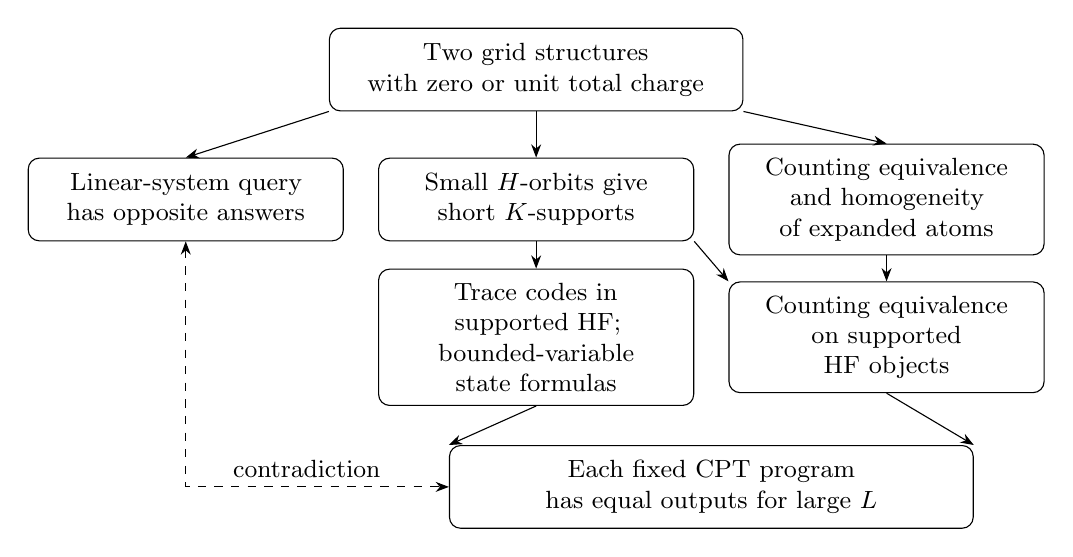
\begin{tikzpicture}[
  >=Stealth,
  box/.style={draw,rounded corners,align=center,font=\small,
              text width=3.65cm,minimum height=1.05cm,inner sep=5pt}
]
\node[box,text width=4.9cm] (input) at (0,0)
  {Two grid structures\\with zero or unit total charge};
\node[box] (query) at (-4.45,-1.65)
  {Linear-system query\\has opposite answers};
\node[box] (support) at (0,-1.65)
  {Small $H$-orbits give\\short $K$-supports};
\node[box] (base) at (4.45,-1.65)
  {Counting equivalence\\and homogeneity\\of expanded atoms};
\node[box] (trace) at (0,-3.4)
  {Trace codes in supported HF;\\bounded-variable\\state formulas};
\node[box] (hf) at (4.45,-3.4)
  {Counting equivalence\\on supported\\HF objects};
\node[box,text width=6.3cm] (equal) at (2.225,-5.3)
  {Each fixed CPT program\\has equal outputs for large $L$};
\draw[->] (input.south west)--(query.north);
\draw[->] (input.south)--(support.north);
\draw[->] (input.south east)--(base.north);
\draw[->] (support.south)--(trace.north);
\draw[->] (support.south east)--(hf.north west);
\draw[->] (base.south)--(hf.north);
\draw[->] (trace.south)--(equal.north west);
\draw[->] (hf.south)--(equal.north east);
\draw[<->,dashed] (query.south) |- 
  node[pos=.73,above,font=\small]{contradiction} (equal.west);
\end{tikzpicture}

\caption{The two routes from the input pair. The charge equations give
opposite query answers. The symmetry, logic and computation arguments
force every fixed choiceless program to give equal answers for sufficiently
large grids. The atom expansions are used only for analysis. If the
program decided $Q$, its equal outputs would contradict the left-hand route.}
\label{fig:proof-map}
\end{figure}

Section~\ref{sec:query} defines the query on all inputs, and
Section~\ref{sec:structures} constructs its two test structures.
Section~\ref{sec:support} proves the support theorem.
Sections~\ref{sec:base-counting} and~\ref{sec:hf-transfer} establish the
counting comparison on atoms and then on supported sets.
Section~\ref{sec:coding} encodes full interpretation computations, and
Section~\ref{sec:separation} fixes the parameters and proves
Theorem~\ref{thm:main}.
Section~\ref{sec:linear-algebraic-logics} proves the definability
of $Q$ in solvability and rank logic.

\section{The grid structures}\label{sec:structures}

The instances used in the lower bound attach finite groups to the edges
of a three-dimensional box.  At each vertex we retain the tuples of edge
states satisfying a prescribed divergence equation.  The group law will
supply the nonabelian automorphisms used in the support argument; the
query just defined will detect an obstruction to the divergence equations.

\subsection{Grid orientations and edge groups}

For an integer $L\ge2$, let $G=(V,E)$ be the box grid with
\[
 V=\{0,\ldots,L-1\}^3.
\]
Each edge is oriented in its positive coordinate direction.  Put
$\epsilon_{ve}=1$ if $v$ is the head of $e$, $\epsilon_{ve}=-1$ if it is
the tail, and $\epsilon_{ve}=0$ otherwise.  The incidence map is
\[
 \partial:\mathbb F^E\longrightarrow\mathbb F^V,
 \qquad (\partial z)_v=\sum_{e\in E}\epsilon_{ve}z_e.
\]
Let $F$ be the set of unit square faces.  A face parallel to coordinate
directions $i<j$ is traversed first in direction $+i$, then $+j$, then
$-i$, then $-j$.  Its edge vector $c^f\in\mathbb F^E$ has coefficient
$1$ when this traversal follows an edge orientation, $-1$ when it opposes
that orientation, and zero off the face.  At each vertex of the face one
traversed edge enters and one leaves, so
\begin{equation}\label{eq:face-cycle}
 \partial c^f=0.
\end{equation}
Write $F(e)=\{f\in F:c^f_e\ne0\}$, and let $F(v)$ be the set of faces
containing $v$.  We shall use
\[
 |F(e)|\le4,\qquad f(v):=|F(v)|\le12,
 \qquad d(v):=|\{e:e\ni v\}|\le6.
\]
In particular, $d(v)\ge1$.

For vectors in $\mathbb F^2$, define the alternating form
\[
 \omega((a,b),(a',b'))=ab'-ba'.
\]
The edge groups use the standard finite Heisenberg multiplication
\cite[Section~2.1]{gurevichHadani2009}, with the face-boundary signs
specifying its alternating form.
The group $P_e$ attached to an edge $e$ has underlying set
$(\mathbb F^2)^{F(e)}\times\mathbb F$.  Its elements are written $(u,z)$,
where $u=(u_f)_{f\in F(e)}$, and its product is
\begin{equation}\label{eq:edge-product}
 (u,z)(u',z')=
 \left(u+u',\ z+z'+\frac12
          \sum_{f\in F(e)}c^f_e\omega(u_f,u'_f)\right).
\end{equation}
Here $1/2=2$ in $\mathbb F_3$.  To verify the group law, denote the
bilinear correction term by $B_e(u,u')$.  Bilinearity gives
\[
 B_e(u,u')+B_e(u+u',u'')
   =B_e(u',u'')+B_e(u,u'+u''),
\]
which is exactly associativity.  Alternation gives $B_e(u,u)=0$; hence
$(0,0)$ is the identity and $(u,z)^{-1}=(-u,-z)$.
In particular, the last coordinate of $(u,z)^{-1}(u',z')$ is
\begin{equation}\label{eq:edge-difference}
 z'-z-\frac12\sum_{f\in F(e)}c^f_e\omega(u_f,u'_f).
\end{equation}

\subsection{Atoms and binary relations}

Fix $b=(b_v)_{v\in V}\in\mathbb F^V$.  The universe of $A_b$ is the
disjoint union of two kinds of atoms.  There is an \emph{edge atom}
$(e,u,z)$ for each edge $e$ and each $(u,z)\in P_e$.  At each vertex $v$
there is a \emph{configuration atom} for every tuple
\[
 a=\bigl(v,((u_e,z_e))_{e\ni v}\bigr)
\]
satisfying
\begin{equation}\label{eq:configuration}
 \begin{aligned}
 u_{e,f}&=u_{e',f}
       &&\text{for the two edges $e,e'$ of each face $f\in F(v)$ at $v$},\\
 \sum_{e\ni v}\epsilon_{ve}z_e&=b_v.
 \end{aligned}
\end{equation}
The coordinates in these descriptions label atoms; they are not members
of the atoms as sets.  The two kinds of atoms are tagged so they are
disjoint.

Figure~\ref{fig:unit-face} illustrates the signed face boundary in
\eqref{eq:face-cycle} and the shared-coordinate condition in
\eqref{eq:configuration}.
\begin{figure}[t]
\centering
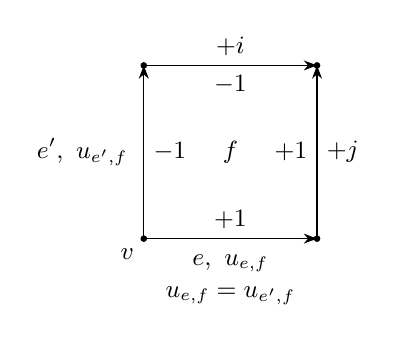
\begin{tikzpicture}[x=1cm,y=1cm,>=Stealth,font=\small]
  \draw[->] (0,0) -- (2.2,0);
  \draw[->] (2.2,0) -- (2.2,2.2);
  \draw[->] (0,2.2) -- (2.2,2.2);
  \draw[->] (0,0) -- (0,2.2);
  \foreach \x/\y in {0/0,2.2/0,2.2/2.2,0/2.2}
    \fill (\x,\y) circle (1.2pt);
  \node[below left] at (0,0) {$v$};
  \node at (1.1,1.1) {$f$};
  \node[above] at (1.1,0) {$+1$};
  \node[left] at (2.2,1.1) {$+1$};
  \node[below] at (1.1,2.2) {$-1$};
  \node[right] at (0,1.1) {$-1$};
  \node[above] at (1.1,2.2) {$+i$};
  \node[right] at (2.2,1.1) {$+j$};
  \node[below] at (1.1,-0.08) {$e,\ u_{e,f}$};
  \node[left] at (-0.08,1.1) {$e',\ u_{e',f}$};
  \node at (1.1,-0.72) {$u_{e,f}=u_{e',f}$};
\end{tikzpicture}

\caption{A geometric grid face $f$ in directions $i<j$. Arrows follow the
global positive-coordinate orientations; the labels $+1,+1,-1,-1$ are
the coefficients of $c^f$, so their signed divergence is zero at each
corner. At the marked vertex $v$, the two incident states of one
configuration satisfy $u_{e,f}=u_{e',f}$. The drawing shows the geometric
cell underlying these coordinates; the atoms are the states and
configurations defined in the text.}
\label{fig:unit-face}
\end{figure}

\begin{lemma}\label{lem:universe-size}
For each $L\ge2$, the size of $A_b$ is independent of $b$ and equals
\begin{equation}\label{eq:universe-size}
 N_L=\sum_{e\in E}3^{2|F(e)|+1}
       +\sum_{v\in V}3^{2f(v)+d(v)-1}.
\end{equation}
In particular,
\[
 L^3\le N_L\le (3^{10}+3^{29})L^3.
\]
Every vertex has at least one configuration atom.
\end{lemma}
\begin{proof}
There are $3^{2|F(e)|+1}$ states on $e$.  At a vertex $v$, each face
$f\in F(v)$ meets precisely two incident edges.  Their face coordinates
are identified by \eqref{eq:configuration}, independently of all other
faces.  The choices of $u$ therefore contribute $3^{2f(v)}$ possibilities.
The divergence condition is a single linear equation in $d(v)$ variables
with a nonzero coefficient, so it has $3^{d(v)-1}$ solutions for every
$b_v$.  This proves \eqref{eq:universe-size} and positivity.  There are
$L^3$ vertices and $3L^2(L-1)\le3L^3$ edges.  The displayed bounds follow
from $|F(e)|\le4$, $f(v)\le12$, and $d(v)\le6$.
\end{proof}

The vocabulary $\tau$ is interpreted as follows; each relation is false
on all pairs not specified below.
\begin{itemize}
\item $\mathsf{Ed}$ and $\mathsf{Cf}$ are the diagonals of the edge atoms
      and configuration atoms, respectively.
\item $\mathsf{EB}$ relates edge atoms on the same edge.  The relation
      $\mathsf{VB}$ relates configuration atoms at the same vertex.
\item $\mathsf I(a,x)$ holds when $a$ is a configuration at a vertex $v$
      and $x=(e,u_e,z_e)$ is the state selected by $a$ on an incident
      edge $e$.
\item For $\delta\in\mathbb F$, the relation
      $\mathsf Z_\delta((e,u,z),(e,u',z'))$ holds precisely when
      \eqref{eq:edge-difference} equals $\delta$.
\end{itemize}
Thus $\mathsf I$ goes from configurations to edge atoms; it is not made
symmetric.  The coordinate labels used to construct $A_b$ are not extra
symbols in its input vocabulary.  In particular, no ordering of the grid
or of its blocks is supplied to a program.

\subsection{Opposite answers}

Fix any vertex $v_*\in V$, and put
\[
 b^0=0,\qquad b^1=\mathbf1_{v_*}.
\]
These two charge vectors give structures of the same size by
Lemma~\ref{lem:universe-size}.

\begin{proposition}\label{prop:opposite-answers}
For every $L\ge2$, the structure $A_{b^0}$ satisfies $Q$ and
$A_{b^1}$ does not.  More generally, $Q(A_b)$ implies
$\sum_{v\in V}b_v=0$ in $\mathbb F$.
\end{proposition}
\begin{proof}
For clarity, let $X(v)$ denote the configuration block at a grid vertex
$v$.  For any $t\in X(v)$, the set $X_t$ in the definition of the query is
exactly $X(v)$.  For an edge atom $y$ on $e$, the test
\eqref{eq:query-incidence-test} holds precisely when $e\ni v$: every
configuration at $v$ selects one atom on each incident edge, and
$\mathsf{EB}$ identifies exactly the edge blocks.  If $e\ni v$, the
coefficient $C(y,a)$ has exactly one contributing selected edge atom,
and exactly one of its three $\mathsf Z_\delta$ relations holds.

On $A_{b^0}$, each vertex has a configuration with all coordinates zero.
Give it weight $\lambda_a=1$ and give all other configurations weight zero.
For $y=(e,u,z)$ set $\mu_y=-z$.  The normalization equations hold.
The selected neighbor of every nonzero-weight configuration on $e$ is
$(e,0,0)$, whose group difference from $y$ has last coordinate $-z$ by
\eqref{eq:edge-difference}.  Thus all equations
\eqref{eq:query-consistency} also hold.

Now suppose the query system on $A_b$ has any solution.  The weights
$\lambda_a$ are arbitrary field elements; we do not assume that they
select a configuration.  For each edge choose, only for this proof, its
zero atom $y_e=(e,0,0)$.  By \eqref{eq:edge-difference}, for $e\ni v$ and
$a\in X(v)$ we have $C(y_e,a)=z_e(a)$.  The equations of the query give
\[
 \mu_{y_e}=\sum_{a\in X(v)}\lambda_a z_e(a),\qquad
 \sum_{a\in X(v)}\lambda_a=1.
\]
Multiply the first identity by $\epsilon_{ve}$, sum over the edges at
$v$, and use \eqref{eq:configuration}:
\[
 \sum_{e\ni v}\epsilon_{ve}\mu_{y_e}
 =\sum_{a\in X(v)}\lambda_a
       \sum_{e\ni v}\epsilon_{ve}z_e(a)
 =b_v\sum_{a\in X(v)}\lambda_a=b_v.
\]
Summing this identity over all vertices cancels each edge contribution,
because an oriented edge has one head and one tail.  Hence
$\sum_v b_v=0$.  For $b=b^1$ that sum is $1$, which is impossible.
\end{proof}

The remainder of the argument shows that a fixed choiceless computation
cannot distinguish these two structures when $L$ is sufficiently large.
The equality of their universe sizes and the fixed binary vocabulary
will be used throughout that argument.

\section{Small orbits have sparse supports}\label{sec:support}

The automorphisms used in this section have two parts. Face translations
form an abelian quotient, but their commutators produce central flows on
edges. This interaction constrains the stabilizer of an object with a small
orbit. We will turn that constraint into a short tuple of atoms whose
pointwise stabilizer in the central flow subgroup fixes the object.

Throughout this section, $\mathbb F=\mathbb F_3$, $L\ge2$, and $G=(V,E)$ is
the positively oriented grid on $\{0,\ldots,L-1\}^3$. Its incidence map is
$\partial:\mathbb F^E\to\mathbb F^V$. For a unit square face $f$, write
$c^f\in\mathbb F^E$ for its oriented boundary, so that $\partial c^f=0$.
Let $F$ denote the set of faces and put
\[
 C_F=(\mathbb F^2)^F,\qquad K=\ker\partial.
\]
We use the alternating form
$\omega((a,b),(a',b'))=ab'-ba'$ on $\mathbb F^2$.

\subsection{A central extension acting on the structures}

For $a,a'\in C_F$, define an edge vector
\[
 B(a,a')=\frac12\sum_{f\in F}\omega(a_f,a'_f)c^f\in K.
\]
On the set $H=C_F\times K$, define
\begin{equation}\label{eq:H-product}
 (a,k)(a',k')=(a+a',k+k'+B(a,a')).
\end{equation}
Bilinearity gives
$B(a,a')+B(a+a',a'')=B(a',a'')+B(a,a'+a'')$, proving
associativity. The identity is $(0,0)$; since $B(a,a)=0$, the inverse of
$(a,k)$ is $(-a,-k)$. Thus $H$ is a finite group. The subgroup
$\{0\}\times K$, identified with $K$, is central, and the projection
$H\to C_F$ is a surjective homomorphism with kernel $K$. With the convention
$[h,h']=hh'h^{-1}(h')^{-1}$, its commutator is
\begin{equation}\label{eq:H-commutator}
 [(a,k),(a',k')]=\left(0,\sum_{f\in F}
                  \omega(a_f,a'_f)c^f\right).
\end{equation}

Recall that an edge atom on $e$ has a state $(u,z)$ in $P_e$, with
$u=(u_f)_{f\in F(e)}$. The element $(a,k)\in H$ sends that state to
\begin{equation}\label{eq:H-edge-action}
 \left(u+(a_f)_{f\in F(e)},\;
 z+k_e+\frac12\sum_{f\in F(e)}c^f_e\omega(a_f,u_f)\right).
\end{equation}
It acts on a configuration by applying this map to every incident edge
state. This is an action because restricting $(a,k)$ to an edge is a
homomorphism from $H$ to $P_e$, and the edge action is left multiplication.

\begin{lemma}\label{lem:H-automorphisms}
For every $b\in\mathbb F^V$, the action just defined is by automorphisms of
$A_b$. On its central subgroup $K$, the action adds $k_e$ to each edge
coordinate $z_e$ and leaves all face coordinates unchanged.
\end{lemma}
\begin{proof}
At a vertex $v$, the two incident coordinates belonging to a face $f$
are equal before the action and both receive the same addition $a_f$.
Hence the face compatibility equations remain true. The change in the
divergence of a configuration is
\[
 (\partial k)_v+\frac12\sum_{f\ni v}
   \left(\sum_{e\ni v}\epsilon_{ve}c^f_e\right)
                        \omega(a_f,u_f).
\]
Here $u_f$ is the common face coordinate in that configuration. Both terms
vanish: $k\in K$ and $\partial c^f=0$. Configurations therefore remain in
the same vertex block and still have divergence $b_v$. Applying the inverse
group element proves bijectivity.

The relations $\mathsf{Ed},\mathsf{Cf},\mathsf{EB},\mathsf{VB}$ are
preserved because types and blocks are preserved. The incidence relation
$\mathsf I$ is preserved because configurations and their specified edge
neighbors are transformed by the same map. Finally, for edge states
$g,g'\in P_e$ and $h\in P_e$, one has $(hg)^{-1}(hg')=g^{-1}g'$.
Consequently every $\mathsf Z_\delta$ is preserved. The formula for the
central action follows from \eqref{eq:H-edge-action} with $a=0$.
\end{proof}

Every permutation of the atoms extends to hereditarily finite objects by
$h\cdot x=\{h\cdot y:y\in x\}$ for sets $x$, recursively in their rank.
Atoms remain distinct from sets. We always use this extension of the
$H$-action. A tuple $\alpha$ of atoms is a \emph{$K$-support} of an object
$x$ if every element of the pointwise stabilizer
\[
 K_\alpha=\{k\in K:k\cdot\alpha_i=\alpha_i\text{ for every }i\}
\]
fixes $x$. The empty tuple is permitted and has stabilizer $K$.

\subsection{A sparse representative for an edge functional}

A central element $k\in K$ fixes an edge atom on $e$ exactly when
$k_e=0$. To obtain a short support for an object $x$, it suffices to find
a small edge set $T$ such that every $k\in K$ vanishing on $T$ fixes $x$.
The stabilizer of $x$ in $K$ is a vector subspace, so it can be described
by linear equations on $K$. We will represent these equations using few
edge coordinates.

An edge cochain is a vector $\ell\in\mathbb F^E$. Its face curl is
\[
 (D\ell)(f)=\sum_e c^f_e\ell_e.
\]
A vertex function $\varphi\in\mathbb F^V$ has gradient
$\partial^{\mathsf T}\varphi$, whose value on an edge from $v$ to $w$
is $\varphi(w)-\varphi(v)$. Adding a gradient does not change the curl,
because $\partial c^f=0$. It also does not change the linear functional
$k\mapsto\sum_e\ell_e k_e$ on $K$.
The next lemma shows that a cochain with few nonzero face curls can be
replaced by one using few edges, without changing its functional on $K$.
In the support proof, commutators
will supply the bound on the number of these faces.

\begin{lemma}[Sparse cochains]\label{lem:sparse-cochain}
Let $\ell\in\mathbb F^E$ have nonzero curl on exactly $t$ faces of the
$L\times L\times L$ box. There is a vertex function $\varphi$ such that
$r=\ell-\partial^{\mathsf T}\varphi$ is supported on at most $2Lt$ edges.
In particular, if $t=0$, then $\ell$ is a gradient.
\end{lemma}
\begin{proof}
We construct the subtracted gradient by successive prefix sums.
Write a vertex as $(i,j,k)$. The cochain coordinate $\ell_1(i,j,k)$ is
on the edge from $(i,j,k)$ to $(i+1,j,k)$, and similarly for directions
$2$ and $3$. Define
\[
 \varphi_1(i,j,k)=\sum_{a=0}^{i-1}\ell_1(a,j,k)
\]
with an empty sum interpreted as zero. Subtracting its gradient produces
a cochain $r^{(1)}$ whose direction-$1$ coordinates vanish. Thus
\begin{align*}
 (D\ell)_{12}(i,j,k)
   &=r^{(1)}_2(i+1,j,k)-r^{(1)}_2(i,j,k),\\
 (D\ell)_{13}(i,j,k)
   &=r^{(1)}_3(i+1,j,k)-r^{(1)}_3(i,j,k).
\end{align*}
Here a subscript $ab$ denotes a face in coordinate directions $a<b$,
and the lower corner ranges over the indices for which the face exists.

Let $t_{ab}$ be the number of nonzero $ab$ curls. The $L$ slices of fixed
first coordinate partition the $23$ faces, so choose $i_0$ for which the
number $t_0$ of nonzero $23$ curls satisfies $t_0\le t_{23}/L$. Put
\[
 \varphi_2(i,j,k)=\sum_{b=0}^{j-1}r^{(1)}_2(i_0,b,k),
 \qquad r^{(2)}=r^{(1)}-\partial^{\mathsf T}\varphi_2.
\]
The function $\varphi_2$ is independent of $i$. Consequently $r^{(2)}_1=0$,
and $r^{(2)}_2(i_0,j,k)=0$. Next put
\[
 \varphi_3(i,j,k)=\sum_{c=0}^{k-1}r^{(2)}_3(i_0,0,c),
 \qquad r=r^{(2)}-\partial^{\mathsf T}\varphi_3.
\]
This last function is independent of $i,j$. We have
\[
 r_1=0,\qquad r_2(i_0,j,k)=0,\qquad r_3(i_0,0,k)=0.
\]
On the slice $i=i_0$, the $23$ curl identity now reads
\[
 r_3(i_0,j+1,k)-r_3(i_0,j,k)=(D\ell)_{23}(i_0,j,k).
\]
It follows that a nonzero value of $r_3$ on this slice must lie after a
nonzero curl on its $j$-line. Each nonzero curl accounts for at most $L$
positions. The slice therefore contains at most $Lt_0$ nonzero edge
coordinates; its direction-$2$ coordinates are all zero. Extending these
slice values constantly across all $L$ slices uses at most
$L^2t_0\le Lt_{23}$ supported coordinates.

The difference between $r_2(i,j,k)$ and $r_2(i_0,j,k)$ is a signed sum of
the $12$ curls between $i_0$ and $i$. Each nonzero $12$ curl can occur in
at most $L$ of these sums. Thus at most $Lt_{12}$ direction-$2$ coordinates
differ from their copied slice values. The identical argument in direction
$3$ gives at most $Lt_{13}$ differing coordinates. Since direction $1$
is zero, the support of $r$ has size at most
\[
 L^2t_0+L(t_{12}+t_{13})\le Lt\le2Lt.
\]
The total subtracted function is
$\varphi=\varphi_1+\varphi_2+\varphi_3$. This construction also covers
$t=0$, when the resulting support is empty.
\end{proof}

\subsection{The support bound}

\begin{proposition}[Small-orbit support bound]\label{prop:small-orbit-support}
Let $N=|A_b|$, let $q\ge0$, and let $x$ be a hereditarily finite object
over the atoms of $A_b$. If its $H$-orbit has size at most $N^q$, then
$x$ has a $K$-support consisting of at most
\[
 2L(q\log_3 N)^2
\]
edge atoms. The support may be empty.
\end{proposition}
\begin{proof}
Let $S=\{h\in H:h\cdot x=x\}$, let $U\le C_F$ be the image of $S$
under the projection, and put $K_0=S\cap K$. Since $C_F$ and $K$ are
additive groups over the prime field $\mathbb F_3$, both $U$ and $K_0$
are vector subspaces. We use the group exact sequence with kernel $K_0$ to obtain
$|S|=|U|\,|K_0|$. Therefore, with
$a=\operatorname{codim}_{C_F}U$ and $d=\operatorname{codim}_K K_0$,
\begin{equation}\label{eq:stabilizer-codimension}
 a+d=\log_3[H:S]\le q\log_3 N=:h.
\end{equation}

Let $W\le K^*$ be the annihilator of $K_0$, so $\dim W=d$. Every
$\lambda\in K^*$ extends to a functional on $\mathbb F^E$, represented
by an edge cochain $\ell$. Two such cochains differ by an element of
$K^\perp=\operatorname{im}\partial^{\mathsf T}$. Indeed that image is
contained in $K^\perp$, and both have dimension $\operatorname{rank}\partial$.

Fix $\lambda\in W$ and a representative $\ell$. For $u,u'\in U$,
choose lifts in $S$. Their commutator lies in $S\cap K=K_0$; evaluating
$\lambda$ on \eqref{eq:H-commutator} gives
\[
 \sum_{f\in F}(D\ell)(f)\,\omega(u_f,u'_f)=0.
\]
Thus $U$ is totally isotropic for the alternating form on $C_F$ with
one block $(D\ell)(f)\omega$ for each face. If $t$ of these coefficients
are nonzero, the form has rank $2t$: a nonzero scalar multiple of
$\omega$ has rank two, and the blocks have disjoint face coordinates
in $C_F$. This rank calculation does not require the boundary vectors
$c^f$ in $K$ to be linearly independent.

We recall the standard dimension argument for alternating forms
\cite[Sections~3.1 and~3.3]{cameron2000classical}.
An alternating form of rank $2t$ on an
$n$-dimensional vector space has no totally isotropic subspace of
codimension less than $t$. Quotient by the radical, of dimension
$n-2t$. The image of an isotropic subspace in this nondegenerate
$2t$-dimensional space has dimension at most $t$, since it is contained
in its orthogonal complement. The original isotropic subspace therefore
has dimension at most $(n-2t)+t=n-t$. Applied above, this shows $t\le a$.
By Lemma~\ref{lem:sparse-cochain}, $\lambda$ consequently has a cochain
representative supported on at most $2La$ edges.

Choose such representatives for a basis of $W$, and let $T\subseteq E$
be the union of their supports. Then
\[
 |T|\le2Lad\le2Lh^2.
\]
This includes $d=0$, when the basis and $T$ are empty. Any $k\in K$
that vanishes on $T$ annihilates every basis member of $W$, hence all
of $W$. Finite-dimensional duality gives $k\in K_0$, so $k$ fixes $x$.
For each edge $e\in T$, choose one edge atom. By the central action,
fixing that atom is equivalent to $k_e=0$. The tuple of chosen atoms
is therefore a $K$-support of $x$ and has the stated length.
\end{proof}

The argument used $x$ only through its stabilizer subgroup $S\le H$.
Its rank plays no role in the support bound.

A family $\mathcal X$ is \emph{membership-transitive} if
$y\in x\in\mathcal X$ implies $y\in\mathcal X$. Thus it contains
every recursive constituent of each of its members.

\begin{corollary}\label{cor:transitive-support}
Let $\mathcal X$ be an $H$-invariant, membership-transitive finite family
of hereditarily finite objects over $A_b$, and suppose
$|\mathcal X|\le N^q$ for some fixed $q\ge0$. Every object in
$\mathcal X$, including every recursive constituent of each of its
members, has a $K$-support of length at most $2L(q\log_3N)^2$.
All these supports can be padded to the common positive length
\begin{equation}\label{eq:support-length}
 s=\left\lceil2L(q\log_3N+1)^2\right\rceil+1
   =O_q\bigl(L(1+\log L)^2\bigr).
\end{equation}
\end{corollary}
\begin{proof}
The orbit of each member is contained in $\mathcal X$, so the proposition
applies to it. Membership transitivity places all its recursive
constituents in the same family. Adding atom coordinates to a support
can only shrink its pointwise stabilizer, so it remains a support.
There are atoms because $L\ge2$; arbitrary atoms can therefore pad even
an empty support. Finally $N=\Theta(L^3)$ gives the asymptotic estimate.
\end{proof}

\section{Counting equivalence and homogeneity}
\label{sec:base-counting}

The central subgroup \(K=\ker\partial\) acts by adding a divergence-free
edge vector to the last coordinates of the atoms.  We now prove two facts
about this action.  First, a bounded number of variables cannot distinguish
the two charge assignments.  Second, within either structure, equality of
sufficiently wide counting types determines a \(K\)-orbit.  The second fact
will let us transport the supports of hereditarily finite sets.

\subsection{An expansion for the analysis}

Recall that an edge atom has coordinates \((e,u,z)\), whereas a configuration
atom at \(v\) specifies the states on all incident edges, subject to the face
compatibility equations and the divergence equation with right side \(b_v\).
Expand \(A_b\) to a structure \(\bar A_b\) as follows.  Partition its universe
into classes indexed by
\[
 (e,u)\quad\text{and}\quad(v,(u_f)_{f\in F(v)}).
\]
Here \(u_f\) is the common face coordinate on the two edges of \(f\) at
\(v\). Thus an edge class leaves only \(z\) unspecified, and a configuration
class leaves all incident \(z\)-coordinates unspecified.  Choose a linear order of
these class labels, the same for all charge assignments, and let
\(\preceq\) be the resulting total preorder on atoms.  Each edge class has
size \(3\), and a configuration class at \(v\) has size
\(3^{d(v)-1}\); in particular, corresponding classes are nonempty and have
the same size.  Finally add, for \(\delta\in\mathbb F_3\), the relation
\[
 \mathsf D_\delta((e,u,z),(e',u',z'))
 \quad\Longleftrightarrow\quad e=e'\ \text{and}\ z'-z=\delta,
\]
which is false on every other pair.  The vectors \(u,u'\) need not agree in
this definition. The preorder will let counting formulas identify a block
and its face coordinates. The relations \(\mathsf D_\delta\) will compare
scalar differences on the same edge, including between different face patterns.

Every element of \(K\) preserves the expansion.  The larger group \(H\)
need not preserve it.  Crucially, the preorder and the relations
\(\mathsf D_\delta\) are tools for this proof and are not part of the input
to a choiceless program.

Write \(C^h\) for first-order logic with equality, ordinary quantifiers and
exact counting quantifiers \(\exists^{=a}x\), using at most \(h\) variable
names.  Here \(a\) may be any nonnegative integer.  Formula length and these
integer constants need not be uniform in \(L\).  The \(C^h\)-type of an
\(r\)-tuple, for \(r\le h\), records all such formulas with free variables
among its \(r\) designated positions.  Coordinates of a tuple may repeat.

\subsection{A component that survives edge deletions}

Let \(G\) be the undirected graph underlying the oriented box grid on
\(V=\{0,\ldots,L-1\}^3\).  For \(R\subseteq V\), write
\(\delta_G R\) for its edge boundary; this notation distinguishes the
boundary of a vertex set from the incidence operator \(\partial\).
The projection estimate below is the three-dimensional discrete
Loomis--Whitney inequality \cite{loomisWhitney1949}.
We include its short proof and derive the needed finite-box boundary bound.

\begin{lemma}[Boundary of a box subset]
\label{lem:box-boundary}
Set \(c=1-2^{-1/3}>0\).  If \(\varnothing\ne R\subseteq V\) and
\(|R|\le L^3/2\), then
\[
 |\delta_G R|\ge c|R|^{2/3}.
\]
\end{lemma}
\begin{proof}
Let \(a_{ij},b_{ik},d_{jk}\) be the indicators of the three coordinate-pair
projections of \(R\).  If their sizes are \(A,B,D\), respectively, then
\[
 |R|\le\sum_{i,j,k}a_{ij}b_{ik}d_{jk}
 \le A^{1/2}\left(\sum_{i,j}
                  \left(\sum_k b_{ik}d_{jk}\right)^2\right)^{1/2}
 \le(ABD)^{1/2}.
\]
For the last inequality apply Cauchy--Schwarz to each inner sum and then
sum the product
\((\sum_k b_{ik}^2)(\sum_k d_{jk}^2)\) over \(i,j\).
Consequently at least one projection has size at least \(|R|^{2/3}\).
It indexes that many nonempty coordinate lines meeting \(R\).  At most
\(|R|/L\) of these lines lie wholly in \(R\).  Every remaining line is a
path meeting both \(R\) and its complement, so contains a boundary edge;
different lines give different edges.  Since
\[
 \frac{|R|}{L}\le 2^{-1/3}|R|^{2/3},
\]
the stated estimate follows.
\end{proof}

Set
\[
 M=\lfloor L^{7/4}\rfloor.
\]
For all sufficiently large \(L\), deleting any set \(T\) of at most
\(6M\) edges leaves a unique component containing more than \(L^3/2\)
vertices.  Call it the \emph{giant component}.  Indeed, summing the preceding
lemma over all components \(R\) of size at most \(L^3/2\) gives
\begin{equation}
\label{eq:small-components}
 \sum_R |R|
 \le c^{-3/2}\sum_R|\delta_G R|^{3/2}
 \le c^{-3/2}(2|T|)^{3/2}
 \le c^{-3/2}(12M)^{3/2}=o(L^3).
\end{equation}
The middle inequality uses \(\sum_R|\delta_G R|\le2|T|\) and
\(\sum_i a_i^{3/2}\le(\sum_i a_i)^{3/2}\) for nonnegative \(a_i\).
If every component had size at most half, the left side would equal
\(L^3\), a contradiction.  Two components cannot both have more than
half the vertices.  Moreover, whenever more edges are deleted within this
range, the new giant is contained in the old one: each new component is
contained in an old component, and its size identifies that old component
as the giant.

\subsection{Moving the unmatched charge}

The counting argument follows the finite-variable counting-game method
of Immerman and Lander \cite[Counting Quantifiers]{immermanLander1990}
and the charge-moving strategy of the CFI construction
\cite[Lemma~6.2 and proof of Theorem~6.4]{cfi1992}.
Here we construct the required bijections and prove formula preservation
directly; no game characterization is needed as a premise.

\begin{proposition}[Base counting equivalence]
\label{prop:base-equivalence}
For all sufficiently large \(L\), the expansions
\(\bar A_{b^0}\) and \(\bar A_{b^1}\), where
\(b^0=0\) and \(b^1=\mathbf1_{v_*}\), satisfy the same \(C^M\) sentences.
\end{proposition}
\begin{proof}
An assigned edge atom touches its edge, and an assigned configuration atom
at \(v\) touches all edges incident with \(v\).  At most \(M\) assigned
positions therefore touch a set \(T\) of at most \(6M\) edges.
Call a paired assignment \emph{compatible} if some vector
\(t\in\mathbb F_3^E\) and some vertex \(w\) in the giant of \(G\setminus T\)
satisfy
\begin{equation}
\label{eq:defect-flow}
 \partial t=b^1-b^0-\mathbf1_w,
\end{equation}
and each assigned atom is paired with the atom obtained by adding \(t_e\)
to its last coordinate on every relevant edge.  This operation leaves its
block and all face-vector coordinates unchanged.  The empty assignment is
compatible with \(t=0\) and \(w=v_*\).

A compatible assignment preserves every atomic formula.  On a fixed edge,
common addition of \(t_e\) preserves both raw differences and the corrected
differences defining \(\mathsf Z_\delta\).  It also preserves whether an
edge state is the specified neighbor of a configuration.  The block
relations, preorder, diagonal predicates and equality are preserved as
well.  This applies even when assigned coordinates repeat.

Deleting an assigned position preserves compatibility: the set of touched
edges shrinks, and the old giant is contained in the new one.  Suppose now
that at most \(M-1\) positions remain.  We construct one bijection of the
entire universes that extends them, regardless of which atom is next
assigned. Its definition may use a different shift on each block; every
such shift will agree with \(t\) on the retained touched edges.
Partition the universe into whole edge blocks and whole vertex
configuration blocks.  For such a block \(J\), let \(T_J\) be \(T\) together
with its edge, or with its vertex star, as appropriate.  There are at most
\(6M\) edges in \(T_J\).  Choose \(w_J\) in the giant of \(G\setminus T_J\).
Both \(w\) and \(w_J\) lie in the giant of \(G\setminus T\), so they are
joined by a path there.  A signed path vector \(p_J\), supported outside
\(T\), can be chosen with
\[
 \partial p_J=\mathbf1_w-\mathbf1_{w_J}.
\]
Put \(t_J=t+p_J\).  It agrees with \(t\) on every previously touched edge
and satisfies \eqref{eq:defect-flow} with \(w_J\) in place of \(w\).

Map every atom in \(J\) by its \(t_J\)-shift.  This gives a bijection on an
edge block.  For a configuration block at \(v\), deleting the star isolates
\(v\), so \(v\ne w_J\).  Hence
\((\partial t_J)_v=b^1_v-b^0_v\), exactly the condition for translation to
map its configurations bijectively to those in the other structure; the
face-vector constraints are unchanged.  The union of these block
bijections is a bijection of universes. For a new atom in block \(J\),
both it and all retained positions are paired by the single shift \(t_J\).
Thus adjoining that atom extends the compatible assignment, with witness
\(t_J,w_J\).

Induct on formulas.  Atomic formulas were handled above, and Boolean
operations preserve agreement.  At a quantifier, first discard any old
assignment of its variable, leaving at most \(M-1\) positions.  The
bijection just constructed pairs all extensions on which the body has the
same truth value by induction.  It therefore preserves ordinary
quantification and every exact counting quantifier, including count zero.
Starting from the empty assignment proves the proposition.
\end{proof}

\subsection{Recognizing the central-group orbits}

For the next step, the two tuples lie in the \emph{same} expansion.  A shift
prescribed on their touched edges must extend to a divergence-free vector.
The only obstruction is a nonzero net prescribed flow across one of the
remaining components.

\begin{lemma}[Extending a partial flow]
\label{lem:partial-flow}
Let \(T\subseteq E\) and \(\sigma\in\mathbb F_3^T\).  There is
\(k\in\ker\partial\) with \(k|_T=\sigma\) if and only if, for every component
\(U\) of \(G\setminus T\),
\begin{equation}
\label{eq:component-balance}
 R_U:=\sum_{v\in U}\sum_{\substack{e\in T\\e\ni v}}
                      \epsilon_{ve}\sigma_e=0.
\end{equation}
If an extension does not exist, there is a nonempty failing component
with
\[
 |U|\le L^3/2,\qquad |U|\le(|T|/c)^{3/2}.
\]
\end{lemma}
\begin{proof}
Extend \(\sigma\) by zero outside \(T\).  The required values on \(E\setminus
T\) must have divergence \(-\partial\sigma\).  On any connected graph, the
image of its incidence operator is exactly the vertex vectors with zero
sum.  To see sufficiency without a rank calculation, take a spanning tree,
set nontree edge values to zero, and eliminate leaves: the divergence at a
leaf uniquely determines the value on its tree edge.  The prescribed total
sum makes the final root equation hold.  Apply this separately to each
component, allowing an isolated vertex as a one-vertex tree.  The necessary
zero-sum conditions are precisely \eqref{eq:component-balance}.

The sum of all \(R_U\) is zero, because the two incidence signs of each edge
cancel.  Thus failure at one component implies failure at at least two, so
one failing component has size at most \(L^3/2\).  Its boundary is contained
in \(T\), and Lemma~\ref{lem:box-boundary} gives the second estimate.
\end{proof}

\begin{proposition}[Quantitative homogeneity]
\label{prop:base-homogeneity}
Let \(r\ge1\), and suppose
\begin{equation}
\label{eq:homogeneity-width}
 7r+7(6r/c)^{3/2}+1\le M.
\end{equation}
If two \(r\)-tuples in the same \(\bar A_b\) have equal \(C^M\)-types, then
some \(k\in K\) maps the first tuple to the second.  The corresponding
statement for empty tuples holds without any width hypothesis.
\end{proposition}
\begin{proof}
Write the tuples as \(\bar a,\bar a'\).  Each preorder class is definable
using two variable names.  If \(h\) is the number of atoms in strictly
earlier classes, its predicate is
\[
 \theta_h(x):=\exists^{=h}y\,
       (y\preceq x\land\neg(x\preceq y)).
\]
Different classes give different \(h\), since every class is nonempty.
Type equality therefore puts corresponding tuple coordinates in the same
class.  They have the same blocks and face-vector patterns.

Let \(T\) be the touched edges, so \(|T|\le6r\).  An \emph{occurrence} of a
state on \(e\in T\) is either an edge atom appearing in a tuple coordinate
or the state on \(e\) in a configuration appearing there.  In the latter
case that state is the unique \(y\) satisfying \(\mathsf I(a_i,y)\) and its
specified edge-class predicate.  The corresponding occurrence for
\(\bar a'\) has the same edge and face-vector coordinates.  For any two
occurrences on one edge, their raw difference can be tested by
\(\mathsf D_\delta\), quantifying their uniquely specified neighbors if
necessary.  These tests use at most the \(r\) tuple names, two neighbor
names, and one name reused in class-counting predicates.  Condition
\eqref{eq:homogeneity-width} in particular permits these \(r+3\) names.
Type equality shows that every pair of corresponding occurrences has the
same raw difference.  Hence there is a single well-defined
\(\sigma_e\) equal to the change in \(z\) from \(\bar a\) to \(\bar a'\)
for all occurrences on \(e\).

Suppose \(\sigma\) cannot be extended to \(K\).  Choose a failing component
\(U\) from Lemma~\ref{lem:partial-flow}; then
\[
 |U|\le(6r/c)^{3/2}.
\]
We construct a formula true at \(\bar a\) and false at \(\bar a'\).
For every \(v\in U\), choose any configuration \(g_v^0\) in the first
assignment's structure and let \(h_{v,e}^0\) be its neighbor on every incident
edge. The chosen configurations need not agree across an internal edge.
The formula will preserve their original raw difference, so any new
witnesses will have equal scalar changes at its two ends. These changes
will cancel when the divergence equations are summed over \(U\).
On each boundary edge \(e\in\delta_GU\subseteq T\), choose one
occurrence from \(\bar a\), and denote its state by \(o_e^0\).  Write
\(o_e\) for the corresponding tuple variable, or the auxiliary neighbor
variable when one is needed.  The formula existentially quantifies
variables \(g_v,h_{v,e}\), and, if the chosen occurrence comes from a tuple configuration,
one neighbor variable \(y_e\).  Its conjunction asserts:
\begin{enumerate}
\item each \(g_v,h_{v,e}\) is in the class of the chosen atom, and
      \(\mathsf I(g_v,h_{v,e})\) holds;
\item for every edge internal to \(U\), the raw difference between its two
      variables \(h_{v,e}\) equals the difference between the two chosen
      atoms \(h_{v,e}^0\);
\item for every boundary edge, the raw difference between \(h_{v,e}\) and
      its chosen tuple occurrence equals their original raw difference;
      if that occurrence requires \(y_e\), also impose its edge-class
      predicate and its incidence with the relevant tuple configuration.
\end{enumerate}
For definiteness, on an internal edge joining \(v,w\), choose an ordering
of its endpoints and use
\[
 \mathsf D_{z(h_{w,e}^0)-z(h_{v,e}^0)}(h_{v,e},h_{w,e});
\]
on a boundary edge incident with \(v\in U\), use
\[
 \mathsf D_{z(h_{v,e}^0)-z(o_e^0)}(o_e,h_{v,e}),
\]
where both atoms in the subscript are the fixed original choices.
Thus \(o_e=y_e\) in the arguments when the occurrence is supplied by a
tuple configuration.
An edge in \(T\) with both endpoints in \(U\) is treated as internal; its
contribution to \(R_U\) cancels and requires no boundary link.
All class predicates are of the form \(\theta_h\) above, and all difference
conditions use one of the three \(\mathsf D_\delta\).  This describes a
finite formula in the expansion's vocabulary; the numerical constants and
its length may depend on the chosen assignments.  The indicated choices
witness its truth at \(\bar a\).

If it were true at \(\bar a'\), compare the realized \(z\)-coordinates of
its witnesses with those of \(h_{v,e}^0\), writing the changes as
\(d_{v,e}\).  Both configurations at \(v\) have divergence \(b_v\), so
\(\sum_{e\ni v}\epsilon_{ve}d_{v,e}=0\).  On an internal edge the difference
constraint gives equal changes at its two ends.  On a boundary edge it
forces \(d_{v,e}=\sigma_e\).  Summing the vertex equations over \(U\)
therefore gives \(R_U=0\), contrary to the choice of \(U\).

There are \(r\) tuple variables, \(|U|\) configuration variables, at most
\(6|U|\) incident-state variables, and at most \(|\delta_GU|\le6r\) extra
occurrence variables.  One further name can be reused in every class
predicate.  Thus the formula uses at most
\[
 r+7|U|+6r+1\le7r+7(6r/c)^{3/2}+1\le M
\]
names, contradicting type equality.  The partial shift therefore extends
to some \(k\in K\), whose action maps every coordinate of \(\bar a\) to the
corresponding coordinate of \(\bar a'\).  For empty tuples take \(k=0\).
\end{proof}

For the support scale used below, fix \(q,m\) first and put
\[
 s=\left\lceil2L(q\log_3 N+1)^2\right\rceil+1,
 \qquad N=\Theta(L^3).
\]
Uniformly for \(1\le r\le\max\{2,m\}s\), the left side of
\eqref{eq:homogeneity-width} is
\[
 O_{q,m}\bigl(L^{3/2}(1+\log L)^3\bigr)=o(L^{7/4}).
\]
Consequently Proposition~\ref{prop:base-homogeneity} applies throughout
that range when \(L\) is sufficiently large. The same choice of \(L\)
ensures \(\max\{4,m+1\}s\le M\), the separate width requirement for
extending atom types in the hereditary-set comparison below.
The exponent \(7/4\) simultaneously ensures \(M^{3/2}=o(L^3)\) for the
giant-component estimate and \(L^{3/2}(1+\log L)^3=o(M)\) for homogeneity
at the support scale. Any fixed exponent strictly between
\(3/2\) and \(2\) would meet these asymptotic requirements.
All these conclusions hold for fixed \(q,m\), chosen before \(L\).

\section{From atom types to hereditarily finite sets}
\label{sec:hf-transfer}

The preceding counting equivalence concerns tuples of input atoms.  A
choiceless computation also constructs sets of atoms, sets of such sets, and
objects of unbounded finite rank.  We now show how small supports let us
transfer bounded-variable counting formulas on a domain containing all these
objects.  The domain itself will be countably infinite; every object in it
is nevertheless hereditarily finite.  The counting argument below respects
this distinction. The support, molecule and form method originates in
Blass, Gurevich and Shelah
\cite[Sections~8--9 of the published version]{bgs1999} and was developed
for counting by Dawar, Richerby and Rossman
\cite[Section~8 of the author version]{drr2008}. We give the full
quantitative argument for the chosen automorphism subgroups and support
bound used here, including exact counts of represented values.

We first isolate the precise hypotheses needed from the preceding sections.
Write $\mathrm{HF}(A)$ for the atoms of $A$ together with all
hereditarily finite sets built from them.
For a finite relational structure $A$, let $\operatorname{tp}_M^A(\bar a)$
be the set of all $C^M$ formulas true at $\bar a$, with free variables among
the indicated tuple positions.  Tuples may have repeated entries.  Two
such types are compared using the same ordered list of variable positions.

\begin{theorem}[Transfer through small supports]
\label{thm:hf-transfer}
Let $A_0,A_1$ be nonempty finite structures in the same binary relational
vocabulary, and let $K_i\leq\operatorname{Aut}(A_i)$ for $i\in\{0,1\}$.
Let $s,m,M$ be positive integers satisfying
\[
 \max\{4,m+1\}s\leq M.
\]
Assume the following two properties.
\begin{enumerate}
\item $A_0$ and $A_1$ satisfy the same $C^M$ sentences.
\item In each $A_i$, any two tuples of length at most
      $\max\{2,m\}s$ with the same $C^M$ type lie in the same $K_i$ orbit.
\end{enumerate}
For $i\in\{0,1\}$, let $D_i$ consist of the objects $x$ in
$\mathrm{HF}(A_i)$ such that $x$ and every object in its transitive closure
have a $K_i$-support of length at most $s$.  Equip $D_i$ with membership,
an atom predicate, and the relations of $A_i$, interpreted as false on
arguments containing a non-atom.  Then $D_0$ and $D_1$ satisfy the same
$C^m$ sentences.
\end{theorem}

Here atoms are urelements, distinct from all sets.  A tuple supports an
object if its pointwise stabilizer fixes that object.  The action of $K_i$
on atoms extends recursively to sets.  We can pad every support to exactly
$s$ coordinates, using repetitions or arbitrary atoms, because $A_i$ is
nonempty.  The resulting domains $D_i$ contain all atoms and all pure
hereditarily finite sets.  They are transitive under membership, countable,
and invariant under $K_i$: if $\alpha$ supports $x$, then $g\alpha$
supports $gx$.

For our application, $A_i$ in Theorem~\ref{thm:hf-transfer} is the analytic
expansion $\bar A_{b^i}$, and $K_i$ is its central flow group $K$.  The base
counting-equivalence and homogeneity results provide its two assumptions
with the parameter bounds established at the end of
Section~\ref{sec:base-counting}. For the remainder of the paper, write
$\mathcal D_{b^i}$ for this supported
domain over $\bar A_{b^i}$, using the support length in
\eqref{eq:support-length}. The atom predicate is definable in our domain by
$\mathsf{Ed}(x,x)\lor\mathsf{Cf}(x,x)$.  No analytic expansion is supplied
to the program; it is used only to prove the indistinguishability theorem.

The proof has three stages: count extensions of atom types; represent
supported objects and transfer equality and membership; then match the
whole domains while retaining the assigned parameters.

\subsection{Exact extension counts for atom types}

All types in the next lemma are realized in $A_0$ or $A_1$.  Thus there are
only finitely many types of any fixed tuple length, even though a type
records infinitely many formulas.

\begin{lemma}[Extension counts]
\label{lem:hf-type-counts}
Suppose $P$ and $P'$ have the same $C^M$ type in two structures chosen,
with repetition allowed, from $A_0,A_1$.  If $|P|+d\leq M$, then for every
realized type $\rho$ of length $|P|+d$, the numbers of tuples $\gamma$
and $\gamma'$ satisfying
\[
 \operatorname{tp}_M(P,\gamma)=\rho,
 \qquad
 \operatorname{tp}_M(P',\gamma')=\rho
\]
are equal.  In particular a type realized over one prefix is realized over
the other.  Equal types also have equal types on every projected or
reordered subtuple.
\end{lemma}

\begin{proof}
Projection and reordering follow by renaming the free tuple variables:
an injection between the selected position sets extends to a permutation
of the $M$ available variable names.  Repeated atom values cause no
problem; positions remain distinct, and equality formulas record all
coincidences of values.

First let $d=1$ and write $a=|P|$.  A realized type $\rho$ of $(a+1)$-tuples
can be isolated among the tuples of both finite structures by a single
$C^M$ formula $\theta_\rho$.  Indeed, choose a representative of $\rho$.
For every tuple in the two structures whose type differs from $\rho$,
choose a formula distinguishing it from the representative, negating the
formula if necessary.  The conjunction of this finite collection is true
exactly on the tuples of type $\rho$.  Its free variables lie among the
first $a+1$ positions, and it still uses only the same $M$ variable names.
If all tuples have type $\rho$, use a tautology.

If exactly $h$ extensions of $P$ realize $\rho$, the formula
\[
 \exists^{=h}x_{a+1}\,
       \theta_\rho(x_1,\ldots,x_a,x_{a+1})
\]
is true at $P$.  Equality of prefix types makes it true at $P'$ as well.
This proves the one-coordinate assertion, including $h=0$ and $a=0$.
For empty prefixes in different structures, the required equality of
types is precisely their agreement on $C^M$ sentences.

For $d>1$, project $\rho$ onto the first $a+d-1$ positions, obtaining
$\sigma$.  By induction the number of extensions of $P$ to type $\sigma$
equals the corresponding number over $P'$.  The one-coordinate argument,
used both within a structure and between the two structures, shows that
every tuple of type $\sigma$ has the same number of last-coordinate
extensions to type $\rho$.  Multiplying these two finite counts proves
the assertion.
\end{proof}

\subsection{A common syntax for supported objects}

A \emph{molecule} is a tuple $\alpha\in A_i^s$.  It records a support, but
need not be a minimal support.  We describe sets by a common collection
of formal expressions, independent of the side $i$.

There are $s$ atomic forms $c_1,\ldots,c_s$.  A set form is a finite set
of pairs $(\psi,\rho)$, where $\psi$ is a previously constructed form
and $\rho$ is a realized $C^M$ type of length $2s$ in $A_0$ or $A_1$.
These are syntactic constructors: atomic forms are distinct from every
set form, including the empty set form.  A form has finite depth; set
forms have greater depth than their constituent forms.

For a molecule $\alpha\in A_i^s$, define the value of a form recursively:
\begin{align}
 c_j*\alpha&=\alpha_j, \label{eq:hf-atomic-form}\\
 \phi*\alpha&=
 \{\psi*\beta:
        (\psi,\rho)\in\phi,
        \ \beta\in A_i^s,
        \ \operatorname{tp}_M^{A_i}(\beta,\alpha)=\rho\}
       \quad\text{if $\phi$ is a set form}.
       \label{eq:hf-set-form}
\end{align}
This produces a finite set because both the form and the base universe
are finite.  The empty set form evaluates to the empty set.

\begin{lemma}[Representation]
\label{lem:hf-representation}
Every value $\phi*\alpha$ belongs to $D_i$ and is supported by $\alpha$.
Conversely, every object of $D_i$ has such a representation.  Moreover,
for every $g\in K_i$,
\[
 g(\phi*\alpha)=\phi*(g\alpha).
\]
\end{lemma}

\begin{proof}
Automorphisms preserve $C^M$ types.  Induction on the form therefore gives
the displayed equivariance identity: in the set case, change the witness
molecule $\beta$ to $g\beta$ in~\eqref{eq:hf-set-form}.  If $g$ fixes
$\alpha$, this identity says that it fixes $\phi*\alpha$.  Induction also
puts every member of a set-form value, and all of that member's recursive
constituents, in $D_i$.  Atomic values have the required support directly.

For the converse, induct on the hereditary rank of the object.  An atom
has the form $c_j*\alpha$ for a molecule containing it.  Let $x$ be a set
in $D_i$, and choose a supporting molecule $\alpha$.  For each $y\in x$,
the induction hypothesis gives $y=\psi_y*\beta_y$.  Form the finite set
\[
 \phi=\{(\psi_y,\operatorname{tp}_M(\beta_y,\alpha)):y\in x\}.
\]
Every member of $x$ lies in $\phi*\alpha$.  Conversely, a member of
$\phi*\alpha$ has the form $\psi_y*\beta$, where
$(\beta,\alpha)$ and $(\beta_y,\alpha)$ have the same type.  Homogeneity
for tuples of length $2s$ supplies an element $g\in K_i$ mapping the
second tuple to the first.  In particular $g$ fixes $\alpha$, so it fixes
$x$.  Equivariance gives $\psi_y*\beta=gy\in x$.  Thus
$x=\phi*\alpha$.  For $x=\varnothing$, the construction gives the empty
set form and the same conclusion.
\end{proof}

Representation reduces arbitrary finite rank to finite syntax.  We next
show that the syntax can be evaluated on either base structure without
changing equality or membership, provided the supporting molecules have
the same joint type.

\begin{lemma}[Transfer of atomic facts]
\label{lem:hf-atomic-transfer}
Let $\phi,\psi$ be forms.  Suppose $(\alpha,\beta)$ and
$(\alpha',\beta')$ have the same $C^M$ type, where the two tuples may be
in the same base structure or in different base structures.  Then
\begin{align*}
 \phi*\alpha=\psi*\beta
   &\quad\Longleftrightarrow\quad
       \phi*\alpha'=\psi*\beta',\\
 \phi*\alpha\in\psi*\beta
   &\quad\Longleftrightarrow\quad
       \phi*\alpha'\in\psi*\beta'.
\end{align*}
The atom predicate and all base relations also agree on corresponding
form values.
\end{lemma}

\begin{proof}
For equality, induct on the sum of the depths of the two forms.  For two
atomic forms, equality is an equality of molecule coordinates and is
recorded by their joint type.  An atomic value never equals a set-form
value.  It remains to compare two set forms.

Suppose $\phi*\alpha=\psi*\beta$.  Take a member of
$\phi*\alpha'$ and a witness for it, say $(\theta,\rho)\in\phi$ and
$\gamma'$ with $\operatorname{tp}_M(\gamma',\alpha')=\rho$.
Lemma~\ref{lem:hf-type-counts} extends the matching prefix
$(\alpha,\beta)$ to a tuple $(\alpha,\beta,\gamma)$ with the type of
$(\alpha',\beta',\gamma')$.  Hence $\theta*\gamma$ is a member of
$\phi*\alpha$, and therefore of $\psi*\beta$.  Choose a witness
$(\xi,\sigma)\in\psi$ and a molecule $\zeta$ such that
\[
 \operatorname{tp}_M(\zeta,\beta)=\sigma,
 \qquad \theta*\gamma=\xi*\zeta.
\]
Apply the extension lemma once more, this time to the primed prefix of
length $3s$, to obtain $\zeta'$ such that
\[
 \operatorname{tp}_M(\alpha,\beta,\gamma,\zeta)
   =\operatorname{tp}_M(\alpha',\beta',\gamma',\zeta').
\]
This is the step requiring $4s\leq M$.  Projection preserves the two
member-witness types.  The induction hypothesis applies to $\theta,\xi$,
whose depths are strictly smaller than those of $\phi,\psi$, and gives
$\theta*\gamma'=\xi*\zeta'$.  Thus the chosen member belongs to
$\psi*\beta'$.  Interchanging $\phi$ and $\psi$ proves the reverse
inclusion.  Finally interchange primed and unprimed data to prove both
directions of equality transfer.  The argument includes empty set forms:
when there is no member to choose, the relevant inclusion is vacuous.

For membership, the right-hand value is either an atom, in which case
membership is false on both sides, or the value of a set form.  In the
latter case, a member witness $\theta*\gamma$ equal to $\phi*\alpha$
can be transferred over the prefix $(\alpha,\beta)$ using $3s$ positions.
Equality transfer, already established for all forms, then transfers the
witness.  Interchanging sides proves the converse.

A form is atomic on both sides or a set form on both sides.  Consequently
the atom predicate transfers.  A base relation is false if any argument
is a set; otherwise it is a relation on selected molecule coordinates,
and its truth is part of their joint base type.  Repeated arguments are
allowed throughout.
\end{proof}

\subsection{Matching entire domains while retaining parameters}

An object may have several representations $\phi*\alpha$. Thus equal
counts of molecules do not by themselves give equal counts of objects.
We will group represented values into stabilizer orbits and account for
the number of molecules representing each value. This will give a
bijection between the two domains after fixing the values of at most
$m-1$ variables. The construction is a mathematical comparison; it is
not required to be definable or executable by a choiceless program.

Call paired assignments \emph{represented alike} if their values have
representations
\[
 x_j=\phi_j*\alpha_j,\qquad x'_j=\phi_j*\alpha'_j
 \quad(1\leq j\leq r),
\]
using common forms, and the concatenated tuples
$P=(\alpha_1,\ldots,\alpha_r)$ and
$P'=(\alpha'_1,\ldots,\alpha'_r)$ have the same $C^M$ type.
Dropping a position preserves this condition by projection.  Empty
assignments are represented alike by the sentence-equivalence assumption.

\begin{lemma}[A bijection extending retained assignments]
\label{lem:hf-bijection}
For any represented-alike assignments with $r\leq m-1$, there is a
bijection $f:D_0\longrightarrow D_1$ such that adjoining any pair
$x,f(x)$ gives represented-alike assignments.  In particular $f(x_j)=x'_j$
for every retained position.
\end{lemma}

\begin{proof}
Fix representing tuples $P,P'$.  A label is a pair $(\phi,\tau)$,
where $\phi$ is a form and $\tau$ is a realized base type of length
$(r+1)s$.  Associate to it the finite value sets
\[
 X_{\phi,\tau}(P)=
   \{\phi*\gamma:\gamma\in A_0^s,
             \ \operatorname{tp}_M(P,\gamma)=\tau\}
\]
and $X_{\phi,\tau}(P')$ on the other side.  The extension-count lemma
shows that the two sets are either both empty or both nonempty.

Every nonempty value set is a single orbit of the stabilizer $K_{0,P}$.
Indeed, any two molecules with the specified type over $P$ are carried
to one another by an element fixing $P$, using homogeneity for
$(r+1)s\leq ms$ positions.  Equivariance carries their values along with
them.  Conversely, an element fixing $P$ preserves the specified joint
type, and thus preserves the value set.  The same assertion holds on the
other side.  It follows that two nonempty label sets on one side either
coincide or are disjoint.

Whether two labels overlap is the same on both sides.  If an overlap has
witnesses $\gamma,\zeta$ on the first side, extend $P'$ to match the type
of $(P,\gamma,\zeta)$.  This uses
\[
 (r+2)s\leq(m+1)s\leq M.
\]
Projection preserves the two label conditions, and
Lemma~\ref{lem:hf-atomic-transfer} preserves equality of the two values.
Hence the label sets overlap on the second side.  The converse is
symmetric.

We also need equality of the sizes of corresponding label sets.  Fix a
nonempty label.  The number $n$ of molecules of its type over $P$ equals
the number over $P'$, by Lemma~\ref{lem:hf-type-counts}.  The map
$\gamma\mapsto\phi*\gamma$ from these molecules onto the label set has
fibres of a common positive size: the stabilizer acts transitively on the
molecules, and equivariance maps one fibre bijectively to another.
Choose molecules $\gamma,\gamma'$ whose joint types with the two prefixes
match.  The fibre at $\phi*\gamma$ has size
\[
 h=\bigl|\{\zeta:
       \operatorname{tp}_M(P,\zeta)=\tau,
       \ \phi*\gamma=\phi*\zeta\}\bigr|.
\]
Partition the possible $\zeta$ by the finitely many realized types of
$(P,\gamma,\zeta)$.  On each such type the two displayed conditions are
constant, both within either structure and between structures: use
projection for the first condition and equality transfer for the second.
Each type has the same number of extensions over $(P,\gamma)$ and
$(P',\gamma')$, again using $(r+2)s\leq M$.  Summing these finite counts
shows that the fibre size $h$ agrees on the two sides.  Both value sets
therefore have size $n/h$.

Representation shows that the label sets cover the domains.  Their
nonempty labels have the same equivalence relation on both sides, where
two labels are equivalent when their value sets overlap.  For each
class, the common value set on the first side and the common value set on
the second side are finite and have equal size.  Choose a bijection
between them.  These bijections combine to a bijection $f:D_0\to D_1$,
because different classes give disjoint value sets.

There are only countably many labels: the base type sets are finite and
the forms are finite expressions over them.  No effective choice is
being assumed here.  For example, fix external enumerations of the two
countable HF universes and of the labels; take the first label of each
class and match its finite value sets in their external enumeration
orders.  These orders belong only to the proof.

If $f$ pairs $x$ with $x'$, a representative label $(\phi,\tau)$ of their
class gives molecules $\gamma,\gamma'$ with
$x=\phi*\gamma$, $x'=\phi*\gamma'$ and common joint type $\tau$ over
$P,P'$.  Thus the extended assignments are represented alike.  If
$x=x_j$ for a retained position, equality transfer forces $x'=x'_j$.
This proves the last assertion as well.
\end{proof}

\begin{proof}[Proof of Theorem~\ref{thm:hf-transfer}]
We prove by induction on $C^m$ formulas that represented-alike assignments
agree on their truth values.  Equality, membership, the atom predicate,
and the input relations agree by Lemma~\ref{lem:hf-atomic-transfer}; for
atomic formulas using two distinct variables, project onto their two
representing molecule blocks.  With one repeated variable, equality is
true and self-membership is false in $\mathrm{HF}$; a diagonal base
relation is false on a set and otherwise is determined by the corresponding
atom coordinate in its molecule type.  Boolean connectives preserve
agreement.

Consider a quantifier binding a variable $x$.  Retain the assigned values
of the other variable names, dropping the old value of $x$ if there is
one.  At most $m-1$ positions remain.  Lemma~\ref{lem:hf-bijection} gives
a bijection of the domains under which every extension by $x$ is again
represented alike.  The induction hypothesis therefore makes this a
bijection between the sets of values satisfying the quantified body.
Existential truth agrees, and for every natural number $h$ the statement
that this set has exactly $h$ elements agrees.  This proves the counting
step even if that set is infinite: a bijection preserves finiteness and
every finite cardinality.  Universal quantifiers follow in the same way
or by negation.  Empty assignments are represented alike, so all $C^m$
sentences have the same truth value.
\end{proof}

Theorem~\ref{thm:hf-transfer} imposes no bound on the rank of an object or
the depth of its representing form. The type-extension arguments require
$4s\leq M$ for equality transfer and $(m+1)s\leq M$ for the domain
bijections. Orbit homogeneity is used at length $2s$ for representation
and at length at most $ms$ when extending a retained assignment.
These requirements are independent of rank. In the next section, the
support theorem places every code and recursive constituent of a
polynomial computation inside $D_i$. We then construct bounded-variable
halt and output sentences evaluated on $D_i$, to which the transfer
theorem applies.

\section{Encoding complete choiceless computations}
\label{sec:coding}

The preceding transfer theorem concerns hereditarily finite sets with small
supports. We now bring an arbitrary fixed choiceless computation into that
setting. There are two separate points to prove: all constituents of its
encoding lie in a polynomial-size invariant family, and its states can be
defined by counting formulas whose number of variable names stays bounded
throughout the computation. For our two inputs, which have the same size,
this will give one common $C^m$ sentence for each stage's halt test and output test, exact
on their supported domains through the respective halt stages, with $m$
depending only on the program.

\subsection{The interpretation characterization}

We use the binary-vocabulary formulation of the interpretation characterization
of choiceless polynomial time with counting, due to Grohe, Schweitzer and
Wiebking~\cite[Section~6 and Theorem~18, arXiv version~1]{gsw2020}, building on
Gr\"adel, Pakusa, Schalth\"ofer and Kaiser~\cite[Theorem~1]{gkps2015}.
Here counting includes the cardinality operation on hereditarily finite sets.
We spell out the exact direction and interpretation convention used below.

An interpretation from one fixed binary relational vocabulary to another
consists of fixed, parameter-free formulas
\[
 \delta(x_1,x_2),\qquad
 \eta(x_1,x_2,y_1,y_2),\qquad
 \rho_R(x_1,x_2,y_1,y_2)
\]
in first-order logic with the H\"artig quantifier. This quantifier compares
the cardinalities of two sets of elements defined by formulas; the two
formulas may have free variables in addition to their respective counted
variables. On a finite structure with universe $V$, the interpretation first
forms
\[
 D=\{(a_1,a_2)\in V^2:\delta(a_1,a_2)\}.
\]
Let $\sim$ be the least equivalence relation on $D$ containing every pair
$(\bar a,\bar b)$ satisfying $\eta(\bar a,\bar b)$. The new universe is
$D/{\sim}$, and
\[
 R([\bar a],[\bar b])
 \quad\Longleftrightarrow\quad
 \text{some }\bar a'\sim\bar a,\ \bar b'\sim\bar b
 \text{ satisfy }\rho_R(\bar a',\bar b').
\]
Thus the interpretation is defined even when $\eta$ itself is not an
equivalence relation or $\rho_R$ is not constant on classes. This is the
convention in~\cite{gsw2020}.

An interpretation program has one such initialization interpretation, one
step interpretation, and fixed halt and output sentences in first-order
logic with the H\"artig quantifier. Write $A_0=A$ for the input,
$A_1=I_{\rm init}(A_0)$, and $A_{j+1}=I_{\rm step}(A_j)$ for $j\ge1$.
The halt sentence is first tested at $A_1$. A deciding program halts at a
stage $h\ge1$, outputs the truth value of its output sentence there, and has
\[
 h+\sum_{j=1}^{h}|V(A_j)|
\]
bounded by a fixed polynomial in $|V(A)|$. The characterization says, in the
direction needed here, that every property of finite binary relational
structures definable in full choiceless polynomial time with counting is
decided by such a program. The absence of parameters means that the fixed
interpretations have no additional input-dependent distinguished tuple;
it does not prohibit free tuple variables in their defining formulas.

Fix a deciding interpretation program $P$. On our two inputs of the same
size $N$, choose a common integer $B\ge2$ bounding $N$, both halt stages,
and every state size up to halt. We may take $B$ to be a fixed polynomial
bound depending only on $P$.

\subsection{A polynomial hereditary encoding}

For objects $a,b$ in the universe of hereditarily finite sets over the input
atoms, use the Kuratowski pair
\[
 \langle a,b\rangle=\{\{a\},\{a,b\}\}.
\]
This coding is injective in the ordered pair, including when $a$ or $b$ is
an atom. Indeed the intersection of its members is $\{a\}$, while their
union is $\{a,b\}$; after recovering $a$, the latter set determines $b$,
also when $a=b$.

Encode the vertices of $A_0$ by the input atoms themselves. Suppose the
vertices of $A_{j-1}$ have already been encoded injectively. A vertex $C$
of $A_j$ is an equivalence class of domain pairs from $A_{j-1}$. Define
its payload and code by
\[
 S_C=\{\langle a_1,a_2\rangle:
       (a_1,a_2)\text{ is a pair of previous codes representing }C\},
 \qquad
 e_j(C)=\langle [j],S_C\rangle,
\]
where $[j]=\{[0],\ldots,[j-1]\}$ is the von Neumann ordinal. Distinct
classes have disjoint, nonempty sets of representing pairs, so their
payloads, and hence their codes, are distinct. The payload records the
whole class, so its construction does not choose a representative. The ordinal tag distinguishes vertices created at
different stages, and stage-zero codes are atoms rather than sets.

\begin{lemma}\label{lem:trace-size}
For either input, the input atoms, all vertex codes up to halt, and all
objects recursively occurring as members of those codes belong to an
$H$-invariant transitive family of at most $9B^3$ objects.
\end{lemma}
\begin{proof}
At a single stage there are at most $B^2$ domain pairs. For each pair,
its Kuratowski code and its two inner sets add at most three objects.
There are at most $B$ classes; their payloads add at most $B$ objects,
and the tagged vertex pairs add at most $3B$ further objects. Previous
vertex codes and their constituents have already been counted. Across
all stages, the ordinal tags and their constituents add at most $B+1$
objects. Including the at most $B$ input atoms, the total is at most
\[
 B(3B^2+4B)+2B+1\le 9B^3
\]
for $B\ge2$. Taking the recursive membership closure therefore gives
the stated transitive family.

Every input automorphism preserves truth of the fixed interpretation
formulas, including the H\"artig quantifier. It therefore permutes the
domain pairs, their generated equivalence classes, and all output
relations. Inductively it permutes the vertex codes: it acts on a pair
or set by acting on its constituents, and fixes every pure ordinal.
It consequently preserves the family and its membership closure.
In particular the input action of $H$ preserves this family.
\end{proof}

Since $B$ is polynomial in $N$, fix an integer $q\ge1$, depending only on
$P$, such that $9B^3\le N^q$ for all sufficiently large $N$. Every
$H$-orbit in the transitive trace family has at most $N^q$ objects.
Corollary~\ref{cor:transitive-support} therefore gives $K$-supports of the
common length $s$ for every code and every recursive constituent. Thus
the entire family lies in the corresponding supported domain
$\mathcal D_b$, including the payloads, all pair wrappers, and the ordinal
tags. No bound on the rank of a code has been imposed: its nesting depth
may grow throughout the computation.

\subsection{Exact formulas for the encoded states}

All formulas in this subsection are evaluated in $\mathcal D_b$ with its
membership relation and its atomic input relations. Its domain is
transitive, contains all input atoms and all pure hereditarily finite sets,
and consists of atoms and sets. Consequently
\[
 \mathsf{Atom}(x):=\mathsf{Ed}(x,x)\vee\mathsf{Cf}(x,x),
 \qquad \mathsf{Set}(x):=\neg\mathsf{Atom}(x)
\]
distinguish these two kinds of objects.

Let $U_0(x)=\mathsf{Atom}(x)$ and let the stage-zero relation formulas be
the input relations. Suppose that the formulas for the preceding stage
are exact: $U(x)$ selects precisely its vertex codes, and its relation
formulas describe exactly the state on those codes. Translate a fixed
first-order formula with H\"artig quantifiers by replacing state relation
atoms by their defining formulas, retaining equality, and restricting
ordinary quantifiers to $U$. In particular, equality is equality of the
injective vertex codes, including for repeated variable arguments.
Replace a H\"artig comparison of $\chi_1(x)$ and $\chi_2(y)$ by
\begin{equation}\label{eq:hartig-translation}
 \bigvee_{n=0}^{B}
 \left[
  \bigl(\exists^{=n}x\,(U(x)\wedge\chi_1^*)\bigr)
  \wedge
  \bigl(\exists^{=n}y\,(U(y)\wedge\chi_2^*)\bigr)
 \right].
\end{equation}
Both counted sets have size at most $B$, so induction on formulas proves
this translation exact, also when the state is empty. The superscript
$*$ will denote this translation.

For the initialization or step interpretation appropriate to the new
stage, put
\[
 \mathsf{Dom}(\bar a):=U(a_1)\wedge U(a_2)\wedge\delta^*(\bar a),
 \qquad \bar a=(a_1,a_2).
\]
On two domain pairs define
\[
 \mathsf{Link}(\bar a,\bar b):=
 \mathsf{Dom}(\bar a)\wedge\mathsf{Dom}(\bar b)\wedge
 \bigl(\bar a=\bar b\vee\eta^*(\bar a,\bar b)
                         \vee\eta^*(\bar b,\bar a)\bigr),
\]
where tuple equality abbreviates the two coordinate equalities. Define
finite formulas recursively by
\[
 \begin{split}
 \mathsf{Reach}_0(\bar a,\bar b)&:=\mathsf{Link}(\bar a,\bar b),\\
 \mathsf{Reach}_{t+1}(\bar a,\bar b)&:=
 \mathsf{Reach}_t(\bar a,\bar b)\vee
 \exists\bar d\,
  (\mathsf{Reach}_t(\bar a,\bar d)\wedge
                         \mathsf{Link}(\bar d,\bar b)).
 \end{split}
\]
This expresses paths of length at most $t+1$ in the reflexive symmetric
link graph. There are at most $B^2$ domain pairs, so
$\mathsf{Reach}_{B^2}$ is exactly the generated equivalence relation,
and is false if either endpoint is outside the domain.

The generated quotient is now defined. We next recognize its hereditary
codes; transitivity will ensure that membership tests identify the actual
sets, not merely their visible members. Write
\[
 \mathsf{Sing}(u,a):=\mathsf{Set}(u)\wedge
                  \forall w\,(w\in u\leftrightarrow w=a),
\]
and
\[
 \mathsf{Double}(v,a,b):=\mathsf{Set}(v)\wedge
               \forall w\,(w\in v\leftrightarrow(w=a\vee w=b)).
\]
Then
\[
 \mathsf{OP}(z,a,b):=
 \exists u\,\exists v\,
 (\mathsf{Sing}(u,a)\wedge\mathsf{Double}(v,a,b)
                         \wedge\mathsf{Double}(z,u,v))
\]
expresses $z=\langle a,b\rangle$ whenever that pair and its wrappers
are present. Conversely every satisfying assignment gives the actual
Kuratowski pair: transitivity ensures that the universally quantified
membership tests cannot overlook a member outside the domain.
Define the ordinal formulas by
\[
 \mathsf{Ord}_i(o):=\mathsf{Set}(o)\wedge
 \forall w\left(w\in o\leftrightarrow
                       \bigvee_{0\le h<i}\mathsf{Ord}_h(w)\right).
\]
The empty disjunction for $i=0$ is false. All pure ordinals belong to
$\mathcal D_b$, and induction using transitivity shows that this formula
selects precisely $[i]$.

For stage $j\ge1$, define
\begin{align*}
 \mathsf{Payload}_j(S,\bar a):={}&
 \mathsf{Set}(S)\wedge\mathsf{Dom}(\bar a)\\[-2pt]
 &{}\wedge\forall z\left(z\in S\leftrightarrow
  \exists\bar b\,
   (\mathsf{Dom}(\bar b)\wedge
    \mathsf{Reach}_{B^2}(\bar a,\bar b)
                      \wedge\mathsf{OP}(z,b_1,b_2))\right),\\
 \mathsf{Rep}_j(x,\bar a):={}&
 \exists o\,\exists S\,
  (\mathsf{Ord}_j(o)\wedge\mathsf{Payload}_j(S,\bar a)
                               \wedge\mathsf{OP}(x,o,S)),\\
 U_j(x):={}&\exists\bar a\,\mathsf{Rep}_j(x,\bar a),\\
 R_j(x,y):={}&\exists\bar a\,\exists\bar b\,
 (\mathsf{Rep}_j(x,\bar a)\wedge\mathsf{Rep}_j(y,\bar b)
                                      \wedge\rho_R^*(\bar a,\bar b)).
\end{align*}
The stage subscripts on the formulas and on their auxiliary definitions
are syntactic indices, not additional free variables.

\begin{lemma}\label{lem:state-exactness}
At every stage through halt, $U_j$ selects exactly the vertex codes of
$A_j$, and each $R_j$ defines exactly its corresponding binary state
relation. The translated halt and output sentences are exact at every
stage $j\ge1$ through halt.
\end{lemma}
\begin{proof}
The assertion at stage zero follows from the definition of the atomic
input relations. Assume it for the preceding stage. Formula induction,
including~\eqref{eq:hartig-translation}, makes $\mathsf{Dom}$ and the
interpretation formulas exact. The link graph and its bounded path
formula therefore give exactly the required classes of domain pairs.

For a domain pair $\bar a$ representing a class $C$, every pair code
belonging to $S_C$ and all its wrappers are in $\mathcal D_b$, by
Lemma~\ref{lem:trace-size} and the support theorem. Hence the right side
of the payload biconditional selects exactly the elements of $S_C$.
The true payload exists in the domain, while any satisfying payload
has exactly those members, since the domain is transitive. Extensionality
for sets gives $S=S_C$. The ordinal and ordered-pair formulas then force
$x=e_j(C)$, with all required witnesses present. This proves the exactness
of $\mathsf{Rep}_j$ and $U_j$. If there are no domain pairs, both formulas
are false for every candidate vertex, as required.

Finally, $R_j$ holds precisely when some representatives of the two
coded classes satisfy the defining relation formula. This is the chosen
quotient semantics, so all relations are exact. Applying the same
formula translation to the fixed halt and output sentences proves the
last assertion.
\end{proof}

\subsection{A variable bound independent of the number of stages}

The formulas just constructed may be extremely long. What matters for
the transfer theorem is a different syntactic bound. For a formula
$\theta$, define
\[
 \operatorname{fw}(\theta)
   :=\max_{\xi\text{ a subformula of }\theta}|\operatorname{FV}(\xi)|.
\]
Here free variables are counted relative to the subformula $\xi$ itself.
Thus a variable bound outside $\xi$ is counted if it occurs freely inside
$\xi$.

\begin{lemma}\label{lem:substitution-width}
Suppose predicates in a relational formula $T$ are replaced by formulas
whose free variables are among their displayed argument variables and
whose free-variable measure is at most $w$. Capture-avoiding substitution
produces a formula of free-variable measure at most
$\max\{\operatorname{fw}(T),w\}$. This allows repeated arguments and
unused displayed argument variables. Moreover a formula of measure at
most $w$ can be renamed to use at most $w+1$ variable names.
\end{lemma}
\begin{proof}
Before each insertion, rename its bound variables to avoid the argument
variables and all possible capture. A subformula inside the inserted
copy has the same free variables as its original counterpart, except
that displayed argument variables are replaced by their actual variable
arguments. This replacement can identify variables but cannot increase
their number. A subformula inherited from the template gains no new
free variables: the inserted formula has free variables only among the
arguments of the atom it replaces. The claimed maximum bound follows.
The argument also covers equality atoms, which are retained as equality,
and atomic occurrences with repeated arguments.

For the renaming claim, fix a palette of $w+1$ names. Recursively process
a formula node with an injective assignment of palette names to that
node's free variables. At a Boolean connective, restrict this assignment
to each child's free variables. At a binder $Qx\,\xi$, keep the assigned
names of the free variables of the parent and choose a name for $x$
outside those names. There is a spare name because there are at most
$w$ parent free variables. If $x$ is free in $\xi$, extend the assignment
by this name; otherwise the binder is vacuous and the child keeps the
parent assignment. Recursively rename the child. Its free-variable
assignment is injective, and its size is at most $w$. Names may be reused
in subtrees where the corresponding variable is not free. This preserves
all bindings and truth, and applies equally to ordinary and exact-count
quantifiers.
\end{proof}

Apply the lemma first to the fixed formulas of $P$. Replacing a
H\"artig quantifier by~\eqref{eq:hartig-translation} may repeat a
subformula $B+1$ times but does not increase its free-variable sets with
$B$; the finitely many program formulas therefore give a uniform bound
for the translation templates. Pair coding, payloads, representatives,
and domain and relation definitions also have fixed templates, with all
free variables among their displayed arguments.

For example, the template for $\mathsf{Reach}_{t+1}(\bar a,\bar b)$
uses only the endpoint pairs $\bar a,\bar b$ and the quantified pair
$\bar d$. The inserted copy $\mathsf{Reach}_t(\bar a,\bar d)$ exposes
only its four endpoint arguments; $\bar b$ occurs in the other conjunct,
$\mathsf{Link}(\bar d,\bar b)$, and is not a free parameter of that
copy. Thus expansion takes the maximum of the previous width and the
fixed template width, rather than adding the widths at successive
levels. The same argument applies when a stage formula is inserted into
the next stage's template. The ordinal recursion has the simpler unary
interface. Taking the maximum over these finitely many template widths
and the bounds for the fixed formulas of $P$ gives a constant $w=w(P)$
for every fully expanded formula above. Unused or identified arguments
can only reduce the number of free variables.

Set $m=\max\{2,w+1\}$. Lemma~\ref{lem:substitution-width} puts all the
expanded state, halt, and output formulas in $C^m$, independently of
$N$, $B$, and the stage number. The numerical constants in the counting
quantifiers and the lengths of these formulas may depend on $B$ and the
stage. These are formulas used to compare two runs; they are not an
additional nonuniform program.

\section{Proof of the separation}\label{sec:separation}

We now combine the invariant query, support bound, counting transfer and
exact computation formulas. The constants controlling supports and formula
width are fixed by the program before the grid is chosen.

\begin{proof}[Proof of Theorem~\ref{thm:main}]
The fixed eight-symbol vocabulary and the query $Q$ are given in
Section~\ref{sec:query}. Proposition~\ref{prop:query-ptime} proves that $Q$
is isomorphism-invariant and belongs to deterministic polynomial time.
Suppose it were definable in full $\CPT$ with counting. The interpretation
characterization in Section~\ref{sec:coding} would give a fixed deciding
interpretation program $P$.

Choose its polynomial bound $B=B(N)$ and the constant $q$
from the trace bound, and choose the constant $m$ from the syntax.
Take $L$ sufficiently large that the trace bound $9B^3\le N^q$ and
the width estimates below hold, and put $M=\lfloor L^{7/4}\rfloor$.
Corollary~\ref{cor:transitive-support} places both encoded traces in
their supported domains with
\[
 s=O_q\bigl(L(1+\log L)^2\bigr).
\]
Proposition~\ref{prop:base-equivalence}
gives base $C^M$ equivalence, and
Proposition~\ref{prop:base-homogeneity} gives homogeneity for tuples of
length at most $\max\{2,m\}s$: its width bound is
$O_{q,m}(L^{3/2}(1+\log L)^3)=o(L^{7/4})$.
We also have $\max\{4,m+1\}s\le M$.
These are exactly the hypotheses of Theorem~\ref{thm:hf-transfer}, so the
two supported domains agree on all $C^m$ sentences.

Use the same $B$, ordinal indices, and syntactic definitions on both
sides. Up to the earlier halt stage both sets of state definitions are
exact. At that stage the common translated halt sentence is true on
one side, hence also on the other; thus both computations halt there.
Their common translated output sentence has the same truth value on
both sides. No deciding interpretation program can therefore give
opposite answers on the two structures.

This contradicts Proposition~\ref{prop:opposite-answers}, which gives
$Q(A_{b^0})$ and $\neg Q(A_{b^1})$ for every $L\ge2$. Therefore no such
program exists, proving the theorem.
\end{proof}

\section{Solvability and rank logic}\label{sec:linear-algebraic-logics}

We now prove the linear-algebraic consequence stated in the introduction.
The query $Q$ is defined on all finite structures. For
Corollary~\ref{cor:linear-algebraic-logics} we take a nonempty input, so
the matrix index sets below are nonempty. We use the two-sorted syntax
of $\mathrm{FPS}_3$ and $\mathrm{FPR}_3$ in
\cite[Section~2]{graedelPakusa2019}.
We first define its matrix without ordering the input, then encode
consistency using the respective operators.

\begin{proof}[Proof of Corollary~\ref{cor:linear-algebraic-logics}]
Write $X(a)$ and $Y(a)$ for the predicates defining $X$ and $Y$, and put
$n=\#x(x=x)$, a closed numeric term. For $\delta=1,2$, the counting terms
\[
 d_\delta(y,a)=\#x\bigl(Y(x)\wedge\mathsf I(a,x)
                         \wedge\mathsf Z_\delta(y,x)\bigr)
\]
give, for each fixed $r\in\{0,1,2\}$, the FPC predicate
\[
 C_r(y,a)\ \equiv\
 \exists\eta\leq 3n\;\bigl(d_1(y,a)+2d_2(y,a)=3\eta+r\bigr).
\]
Here $\eta$ is a number variable. Since $d_1+2d_2\leq3n$, this says
exactly that $C(y,a)=r$ in $\mathbb F_3$. It includes both contributions
when $\mathsf Z_1$ and $\mathsf Z_2$ both hold, while $\mathsf Z_0$
contributes zero. The row test is the first-order predicate
\[
\begin{split}
 T(t,y)\ \equiv\ X(t)\wedge Y(y)\wedge\exists a\,\exists x\,
 \bigl(&X(a)\wedge\mathsf{VB}(t,a)\wedge Y(x)\\
       &{}\wedge\mathsf I(a,x)\wedge\mathsf{EB}(y,x)\bigr).
\end{split}
\]

For nonempty $A$, use the full tuple domain $D=A^2\times\{0,1\}$ for both
rows and columns, with the last coordinate in the number sort. For
$i=(t,y,\rho)$ and $j=(a,z,\kappa)$, define
\[
\begin{aligned}
 N(i)&\equiv \rho=0\wedge t=y\wedge X(t),&
 E(i)&\equiv \rho=1\wedge T(t,y),\\
 L(j)&\equiv \kappa=0\wedge a=z\wedge X(a),&
 U(j)&\equiv \kappa=1\wedge a=z\wedge Y(a).
\end{aligned}
\]
Set $b_i=\mathbf{1}_{N(i)}$ and, over $\mathbb F_3$, set
\[
 M_{ij}=
 \begin{cases}
 1&N(i)\wedge L(j)\wedge\mathsf{VB}(t,a),\\
 -C(y,a)&E(i)\wedge L(j)\wedge\mathsf{VB}(t,a),\\
 1&E(i)\wedge U(j)\wedge a=y,\\
 0&\text{otherwise}.
 \end{cases}
\]
The tags make these cases disjoint. The diagonal payloads give one column
for each $\lambda_a$ and one separately tagged column for each $\mu_y$,
even when $X$ and $Y$ overlap. They also give one normalization row for
each $t\in X$, while the $E$ rows retain every selected pair $(t,y)$.
All remaining rows and columns are zero, with right-hand side zero on
those rows. Thus $Mx=b$ is exactly the system defining $Q$, with harmless
zero padding. In particular an empty $X_t$ still gives $0=1$.
The predicates $B_r(i,j)\equiv(M_{ij}=r)$ for $r=1,2$ are FPC-definable
from these cases and $C_1,C_2$.

The solvability operator uses a Boolean matrix and an all-ones
right-hand side; compare the general fixed-ring normal form in
\cite[Lemma~4.1]{dghkp2013}. For an explicit encoding here, use full row
and column domains $D\times\{0,1,2,3\}$, with column tags denoting
$x^1_j,x^2_j,z_j,v_j$. For every $i\in D$, the four row tags encode
\[
\begin{gathered}
 \sum_{j:B_1(i,j)}x^1_j+
 \sum_{j:B_2(i,j)}(x^1_j+x^2_j)+\mathbf{1}_{\neg N(i)}v_i=1,\\
 v_i=1,\qquad x^1_i+z_i=1,\qquad x^2_i+z_i=1.
\end{gathered}
\]
All coefficients are zero or one: the two summands for $B_2$ use distinct
columns. Their incidence is one FPC formula using $B_1,B_2,N$, equality
of tuples in $D$, and the fixed numeric tags. Every row in the full
product has one of the four stated types. The last two equations force
$x^1=x^2$; together with $v=1$, the first equations then say $Mx^1=b$.
Conversely, a solution $x$ of $Mx=b$ extends by
$x^1=x^2=x$, $z=1-x$, and $v=1$. Hence one characteristic-three
solvability operator defines $Q$.

For rank, let $\mathbf{1}_\psi$ denote the numeric counting term
$\#\zeta\leq0.\psi$, where $\zeta$ is a number variable, and put
$m(i,j)=\mathbf{1}_{B_1(i,j)}+2\mathbf{1}_{B_2(i,j)}$.
On rows $D$ and columns $D\times\{0,1\}$, with numeric tag $h$, use the
entry terms
\[
\begin{aligned}
 \Theta_0(i;j,h)&=\mathbf{1}_{h=0}m(i,j),\\
 \Theta_+(i;j,h)&=\Theta_0(i;j,h)+\mathbf{1}_{h=1\wedge N(i)}.
\end{aligned}
\]
The first matrix is $M$ with zero columns; the second adjoins one copy
of $b$ for each $j\in D$. Since $D$ is nonempty, those identical copies
span the same space as one augmented column. The rank operator reduces
numeric entries modulo three, so
\[
 Q(A)\quad\Longleftrightarrow\quad
 \operatorname{rk}_3(\Theta_0)=\operatorname{rk}_3(\Theta_+).
\]
All domains used above are permitted Cartesian products with fixed
numeric bounds; none chooses or orders an input element.

Finally, the proof of Theorem~\ref{thm:main} uses only the nonempty
witnesses with $L\geq2$, so these definitions prove both noncontainments.
The empty input remains a true instance of $Q$ under its definition in
Section~\ref{sec:query}.
\end{proof}

\clearpage
\bibliographystyle{plain}
\bibliography{references}
\end{document}
